%
% this file is encoded in utf-8
% v1.7
\chapter{模擬結果數值討論與分析}
\section{模擬環境參數設定}
為呈現所提出的排程演算法的成效,本碩士論文採用由Piro等人所提出並被廣泛使用的LTE-Sim\cite{ltesim2011}的Release 5版本作為模擬環境,並設定為單細胞的模擬環境,如圖 \ref{fig:Sim_Environment}所示,而相關的環境參數設定參見表 \ref{tab:Sim_parameters}。環境參數的設定參考\cite{ltesim2011}、\cite{ahme2016}。在基地台半徑1公里的範圍內,使用10 MHz的頻寬,其中每個資源區塊包含12個子載波,每個資源區塊使用180 KHz的頻寬,在10 MHz中總共50個的資源區塊。我們記錄模擬時間共100秒內的封包傳輸狀況,每一個傳輸時間間隔為1 ms,使用者裝置的數量從10個開始,依每次間隔10個遞增至130個,於模擬初期的使用者之間距離為均勻分布的方式隨機配置在基地台所在的單細胞中,模擬過程中每個使用者移動的模型為隨機方向的移動,使用的調變編碼技術為四階相位移鍵、十六階正交波幅調變、六十四階正交波幅調變。為盡量降低隨機性對結果的影響,我們增加使用不同隨機種子進行模擬的次數,每個不同使用者裝置數量的環境都透過不同的隨機種子模擬20次,各項結果為20次模擬結果的平均值。用於UFS中的分配量門檻值$\mathcal{A}_T$,經過多組實驗後選擇使用3做為分配量門檻值。

\begin{table}[H]
\centering
\caption{模擬環境參數表。}
\vskip 10pt
\label{tab:Sim_parameters}
\begin{tabular}{lllll}
\textbf{Parameter}       &  &  &  & \textbf{Value}   \\ \thickhline
Simulation Environment   &  &  &  & LTE-Sim Release 5\\
Simulation Duration      &  &  &  & 100 s            \\
Numbers of Seeds         &  &  &  & 20               \\
Cell Radius              &  &  &  & 1 km             \\
Bandwidth                &  &  &  & 10 MHz           \\
Resource Block Bandwidth &  &  &  & 180 KHz          \\
Subcarriers per Resource Block &  &  &  & 12         \\
Transmission Time Interval (TTI)&  &  &  & 1 ms      \\
Number of UEs            &  &  &  & 10 - 130         \\
Number of RBs (per TTI)  &  &  &  & 50               \\
User Transmit Power		 &  &  &  & +23 dBm          \\
User Mobility Model		 &  &  &  & Random Direction \\
Users Distance Distribution&  &  &  & Uniformly Distributed \\
Modulation Schemes       &  &  &  & QPSK, 16-QAM, 64-QAM \\
Threshold of Allocation Amount $\mathcal{A}_T$     &  &  &  & 3 \\
VoIP Bit Rate            &  &  &  & 12.8 kbps      	 \\
Video Bit Rate           &  &  &  & 242 kbps         \\
Web Bit Rate             &  &  &  & 10 kbps          \\
VoIP Max Delay           &  &  &  & 100 ms           \\
Video Max Delay          &  &  &  & 150 ms           \\
Web Max Delay            &  &  &  & 300 ms           \\ \thickhline
\end{tabular}
\end{table}

在服務流的方面,我們參考在\cite{ltesim2011}、\cite{ahme2016}中對於三種不同的服務流的設定,分別為VoIP、Video、Web,其中的VoIP和Video屬於保證位元速率類型的即時性服務流,而Web則屬於不保證位元速率類型的非即時性服務流,VoIP服務流的傳輸速率為12.8 kbps且型態為G.729;Video服務流的傳輸速率為242 kbps且型態為H.264;Web服務流的傳輸速率為10 kbps而型態為網路傳輸。不同於許多的研究中在非即時性服務流採用的盡力服務(Best Effort)型態,因為盡力服務服務流為一種理想的服務流,於每一次的傳輸時間間隔決定此次要傳輸的資料量大小,然後才產生封包進行傳輸,無法取得封包延遲進行計算,因此,本碩士論文採用模擬網路使用狀況的Web服務流做為非即時性服務流。但是,在\cite{ltesim2011}、\cite{ahme2016}中並未特別描述不同種類的服務流所使用的延遲預算,因此,我們參考\cite{QCI_spec}中長期演進所定義的服務品質識別表 \ref{tab:QoS},依照服務品質等級識別指標1、指標2、指標6,依序設定VoIP、Video、Web三種服務流的延遲預算各別為100 ms、150 ms、300 ms。除了服務流種類上的設定,我們也同時針對兩種不同的模擬環境下進行模擬,分別為固定的服務流數量以及隨機的服務流數量。大多數的研究在模擬環境設定上,都是將使用者裝置中的服務流控制在固定的數量,但是,在實際的情況中,每一個使用者裝置並不一定皆擁有固定種類的服務流需要服務,因此,我們除了讓每個使用者裝置都有固定數量的服務流環境,也對隨機給予使用者裝置不同種類的服務流數量的環境進行模擬;我們採用離散型均勻分布(Discrete Uniform Distribution)的方式,給予使用者裝置不同種類的服務流,每個使用者裝置中,同一種服務流最多為一個,最少為零個;同時,為了確保每一個使用者裝置都處於主動(Active)的狀態,若使用者裝置沒有被分配VoIP和Video服務流時,則會至少分配一個Web服務流來確保使用者裝置可以維持在啟動的狀態。我們在這兩種使用者裝置擁有不同的服務流數量配置環境下,分別比較不同排程演算法的效果差異,並對模擬的結果,從四種不同方面的效果來對排程演算法進行分析,分別為端點對端點延遲(End-to-End Delay)、封包遺失率、公平性以及吞吐量。

\vskip 30pt
\begin{figure}[H]
\centering
\includegraphics[%
  	scale=0.2,keepaspectratio]{figure/Simulation_Environment}
\caption{\label{fig:Sim_Environment}模擬環境示意圖。}
\end{figure}
\begin{comment}
\begin{figure}[H]
\centering
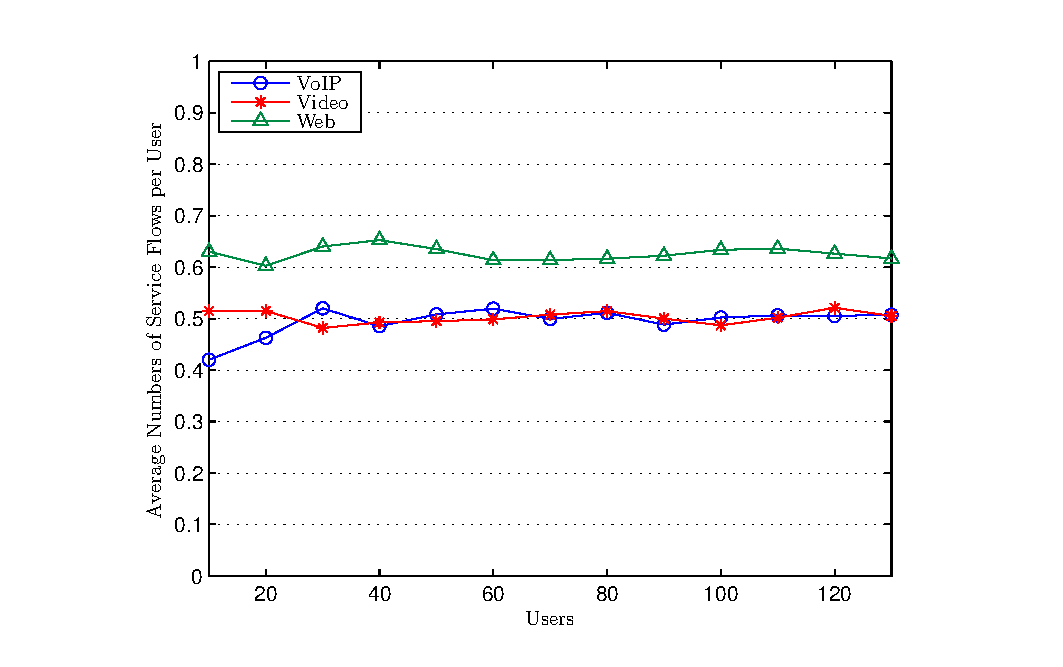
\includegraphics[%
  	scale=0.7,keepaspectratio]{figure/Flows/Flows_avg}
\caption{\label{fig:Flow_avg}隨機服務流數量下使用者裝置平均服務流數量圖。}
\end{figure}
\begin{figure}[H]
\centering
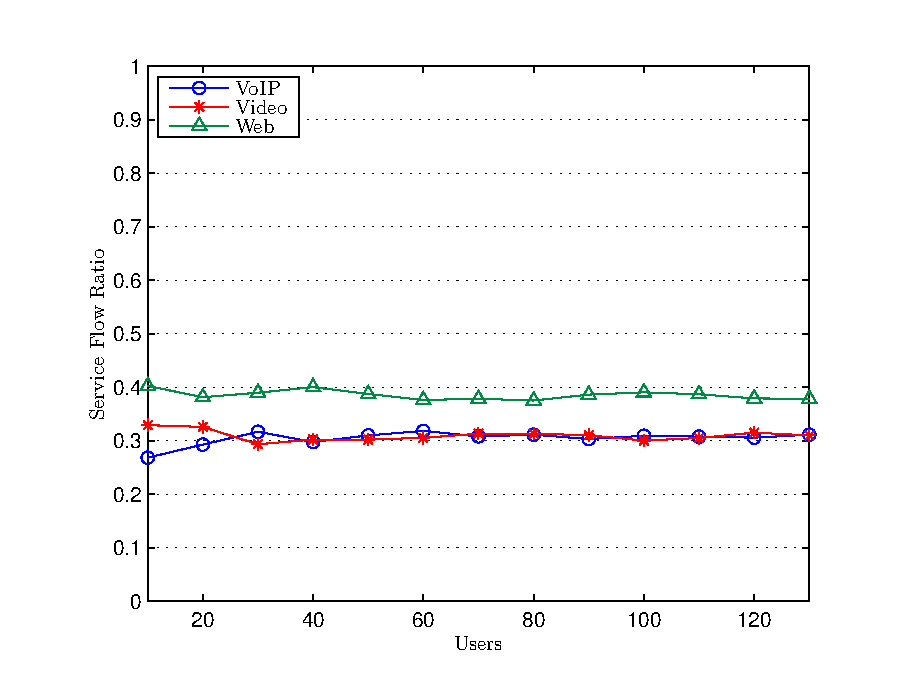
\includegraphics[%
  	scale=0.7,keepaspectratio]{figure/Flows/Flows_ratio}
\caption{\label{fig:Flow_ratio}隨機服務流數量下各服務流所佔比例圖。}
\end{figure}
\begin{figure}[H]
\centering
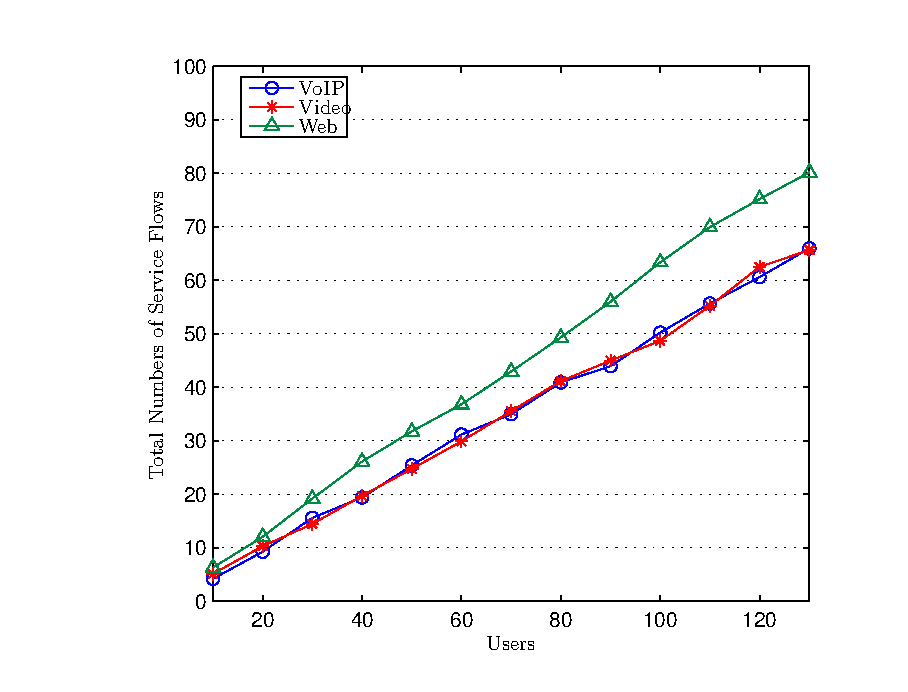
\includegraphics[%
  	scale=0.7,keepaspectratio]{figure/Flows/Flows_numbers}
\caption{\label{fig:Flow_numbers}隨機服務流數量下各服務流數量圖。}
\end{figure}
\end{comment}
\clearpage
\section{加權公平性}
在模擬環境中我們使用三種不同的服務流模擬資料傳輸的狀況,分別有兩種即時性與一種非即時性服務流,但是這三種服務流所能產生的吞吐量不同,在計算使用者裝置之間的公平性時需要給予其不同的權重。在固定的服務流數量下,每個使用者裝置在三種不同的服務流上都各自擁有同樣數量的服務流,在計算彼此之間的公平性時,每個使用者裝置不需要另外加上權重;而在隨機的服務流數量下,每個使用者裝置在三種服務流上所擁有的服務流數量不同,不同使用者裝置自身的吞吐量會產生差異,因此,由Jain等人所提出的普遍被使用於表示公平性的珍式公平性指標(Jain's Fairness Index)\cite{jain1984}僅適用於本碩士論文中使用的固定服務流數量模擬環境,而不完全適用於另外提出的隨機服務流數量模擬環境,珍式公平性指標的計算方式如公式(\ref{Jain})所示,其中$T_n$代表使用者裝置$n$的總吞吐量,$\mathcal{N}$為使用者裝置總數,
\begin{equation}
\label{Jain}
J=\dfrac{\Bigg[\sum\limits_{n=1}^\mathcal{N} T_n\Bigg]^2}{\mathcal{N}\times\Bigg[\sum\limits_{n=1}^\mathcal{N}{T_n}^2\Bigg]}
\end{equation}

而根據\cite{ferng2009},在計算公平性時,由於不同種類的服務流能產生的吞吐量並不相同,VoIP與Video服務流能產生的吞吐量便相差許多,因此,在計算兩者之間的公平性時必須要給予其不同的權重,再進行公平性的計算。於\cite{ferng2009}中提出三種不同層級觀察公平性時所使用的加權計算方式,分別為相同服務流之間、不同服務流之間與不同使用者裝置之間,其中不同使用者裝置之間對於使用者裝置$i$所使用的加權值$w_i$計算方式如公式(\ref{weight})所表示,
\begin{equation}
\label{weight}
w_i=\dfrac{\sum_l\sum_jK_{j,l}^i}{\sum_i\sum_l\sum_jK_{j,l}^i}
\end{equation}
其中$K_{j,l}^i$代表使用者裝置$i$中服務流種類$l$下的第$j$個服務流的期望吞吐量。在本碩士論文中,隨機服務流數量的環境下,每種服務流的數量最多只會有1個,最少為0個存在於使用者裝置內,因此,可以將公式(\ref{weight})改寫如下表示:
\begin{equation}
\label{simple_weight}
w_i=\dfrac{\sum_l\delta(i,l)K_l^i}{\sum_i\sum_l\delta(i,l)K_l^i}
\end{equation}
其中$K_l^i$代表使用者裝置$i$中服務流種類$l$的期望吞吐量,$\delta(i,l)$表示使用者裝置$i$中是否存在服務流種類$l$,如果使用者裝置$i$中存在服務流種類$l$,則$\delta(i,l)=1$,反之,則$\delta(i,l)=0$。透過公式(\ref{simple_weight})計算出$w_i$後,便可以將各使用者裝置的加權值$w_i$加入公式(\ref{Jain}),將其改寫成計算適用於評估本碩士論文中隨機服務流數量環境下$\mathcal{N}$個使用者裝置間的整體公平性$F_I$,其中的$T_i$為使用者裝置$i$模擬結果的實質吞吐量。
\begin{equation}
\label{fairness_index}
F_I=\dfrac{\Bigg[\sum\limits_{i=1}^\mathcal{N}\dfrac{T_i}{w_i}\Bigg]^2}{\mathcal{N}\times\Bigg[\sum\limits_{i=1}^\mathcal{N}\Big(\dfrac{T_i}{w_i}\Big)^2\Bigg]},
\quad 0\leq F_I\leq 1
\end{equation}

公平性$F_I$會是一個介於0與1之間的正數,$F_I$越靠近0則表示公平性越低落,使用者裝置之間加權過後的吞吐量差異越巨大,資源可能集中在部分使用者裝置上而可以有較多的吞吐量;若$F_I$越靠近1則可以說明使用者裝置之間的公平性越高,加權過後的吞吐量的差異並不多,使用者裝置都能獲得足夠的資源以傳輸資料。
\section{植基於急迫性之公平排程法分析}
我們所提出的排程演算法UFS主要考量使用者裝置的急迫度與平均配置資源度,同時在資源區塊的連續分配上加入調變編碼技術限制。將使用者裝置的急迫度、平均配置資源度與調變編碼技術限制這三種考量加入排程演算法的原因與希望達到的效果皆不相同,加入急迫度是希望能減少封包在佇列中因為超過延遲預算而被丟棄的機率,平均配置資源度則是用來增加過去拿到相對較少資源的使用者裝置能優先拿到資源的機率,最後,調變編碼技術限制讓連續分配時可以提高資源區塊的使用效率與更多使用者裝置可以分配到資源的機率。本節將比較UFS中所考量的急迫度、平均配置資源度與連續分配時的調變編碼技術限制各自帶來的影響,同時,討論在公式(\ref{Priority})中使用不同指數數值的$\mu$與$\nu$時,分別在端點對端點延遲、封包遺失率、公平性與吞吐量上的影響。
\clearpage
\subsection{優先權值指數選擇}
在UFS中,用於決定使用者裝置取得資源優先順序的公式(\ref{Priority})中,可以利用$\mu$與$\nu$分別調整急迫度$U_i(t)$與平均配置資源度$\overline{A_i(t)}$對優先權值$P_i(t)$的影響程度。在公式(\ref{Priority})中,急迫度$U_i(t)$做為主要影響優先權值$P_i(t)$的主要原因,平均配置資源度$\overline{A_i(t)}$則做為輔助急迫度的權值。為了進一步了解調整指數$\mu$與$\nu$對優先權值$P_i(t)$的影響,我們將使用以下不同的數值帶入公式(\ref{Priority})中:
\begin{equation}
\left . 
\begin{array}{l} 
\mu=1,\nu=0
 \\ 
\mu=0,\nu=1
 \\ 
\mu=1,\nu=1
 \\ 
\mu=0.5,\nu=1
 \\ 
\mu=1.5,\nu=0.5
\end{array}\right .
\end{equation}
在指數數值的選擇上,我們除了討論各自單獨使用急迫度或平均配置資源度決定使用者裝置分配資源的優先順序的情形外,我們也在$0\leq\mu\leq 2$與$0\leq\nu\leq 1$的範圍內討論幾組不同的數值,找出不同程度的急迫度與平均配置資源度影響使用者裝置優先順序的結果。我們可以透過圖 \ref{fig:UFS_delay_voip}、圖 \ref{fig:UFS_delay_video}、圖 \ref{fig:UFS_delay_web}、圖 \ref{fig:UFS_PLR}、圖 \ref{fig:UFS_Fairness}、圖 \ref{fig:UFS_Throughput}觀察使用不同的$\mu$與$\nu$調整急迫度$U_i(t)$與平均配置資源度$\overline{A_i(t)}$對優先權值$P_i(t)$在端點對端點延遲、封包遺失率、公平性與吞吐量上的影響。
\begin{comment}
\begin{figure}[H]
\centering
\subfigure[\label{fig:UFS_fix_delay}固定服務流數量UFS使用不同指數時的整體端點對端點延遲。]{
 	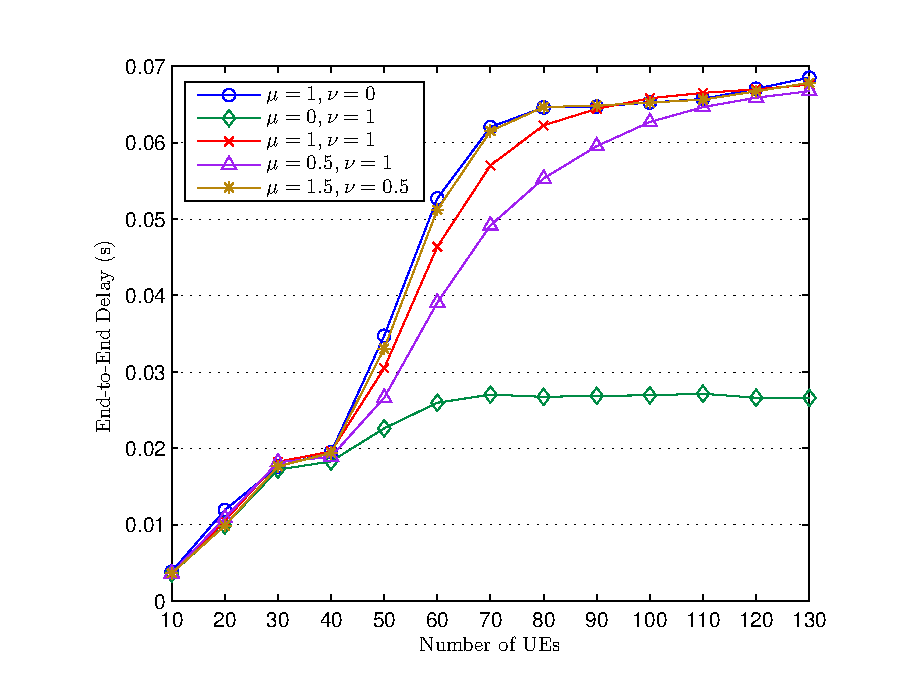
\includegraphics[%
  	scale=0.7,keepaspectratio]{figure/UFS/fixed/Delay}
}
\subfigure[\label{fig:UFS_ran_delay}隨機服務流數量UFS使用不同指數時的整體端點對端點延遲。]{
	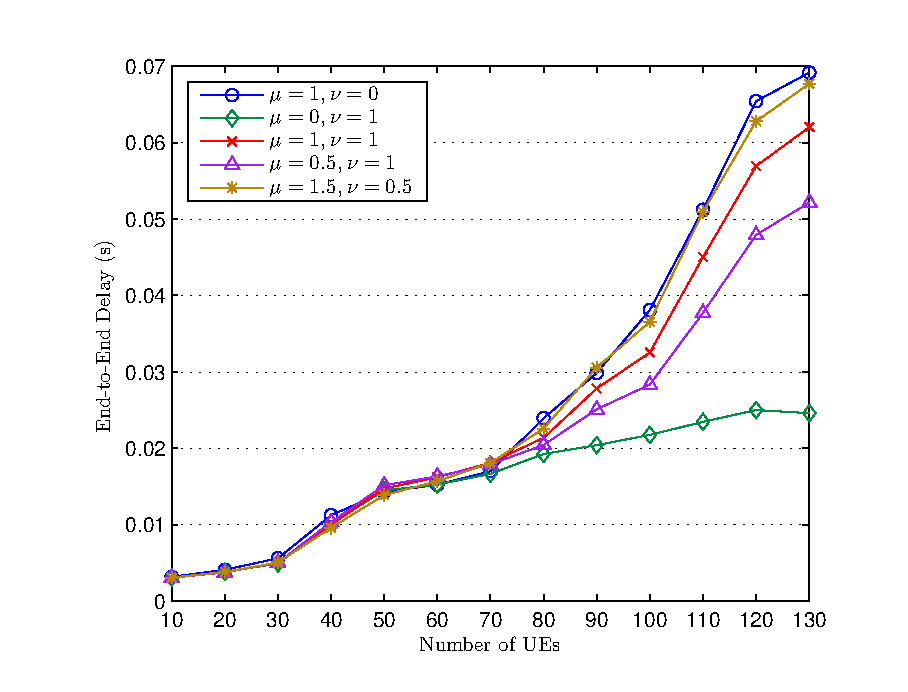
\includegraphics[%
	scale=0.7,keepaspectratio]{figure/UFS/random/Delay}
}
\caption{\label{fig:UFS_delay}不同環境中UFS使用不同指數時的整體端點對端點延遲。}
\end{figure}
\end{comment}
\begin{figure}[H]
\centering
\subfigure[\label{fig:UFS_fix_delay_voip}固定服務流數量下UFS使用不同指數時VoIP的端點對端點延遲。]{
 	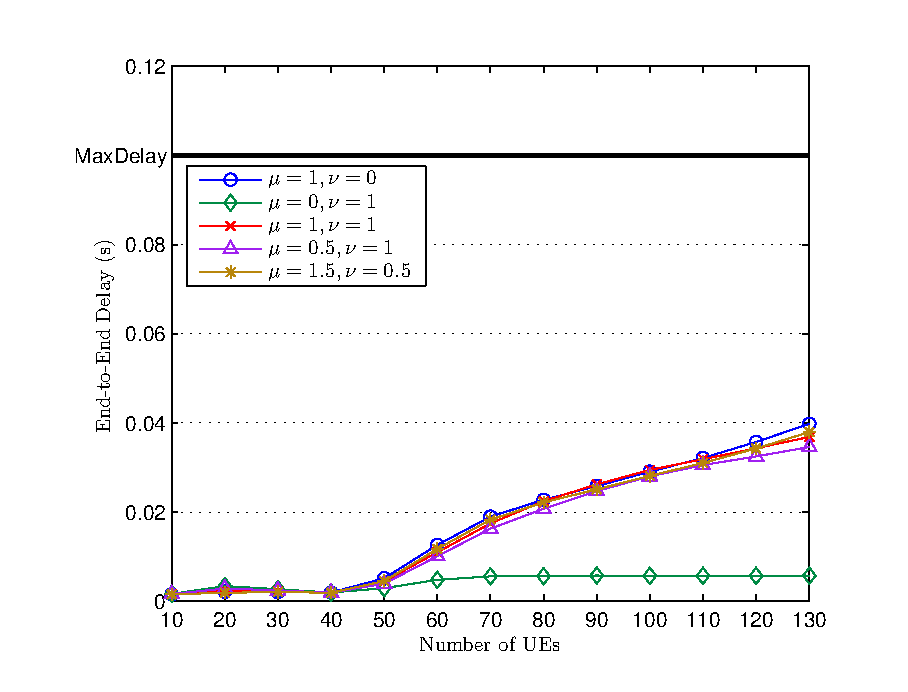
\includegraphics[%
  	scale=0.7,keepaspectratio]{figure/UFS/fixed/Delay_VoIP}
}
\subfigure[\label{fig:UFS_ran_delay_voip}隨機服務流數量下UFS使用不同指數時VoIP的端點對端點延遲。]{
	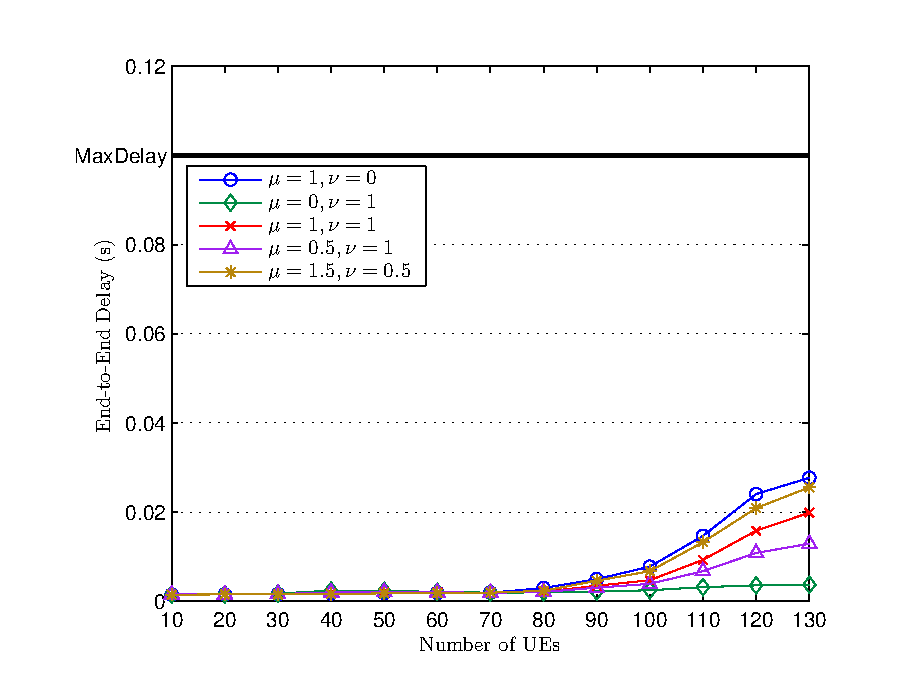
\includegraphics[%
	scale=0.7,keepaspectratio]{figure/UFS/random/Delay_VoIP}
}
\caption{\label{fig:UFS_delay_voip}不同環境中UFS使用不同指數時VoIP服務流的端點對端點延遲。}
\end{figure}
\begin{figure}[H]
\centering
\subfigure[\label{fig:UFS_fix_delay_video}固定服務流數量下UFS使用不同指數時Video的端點對端點延遲。]{
 	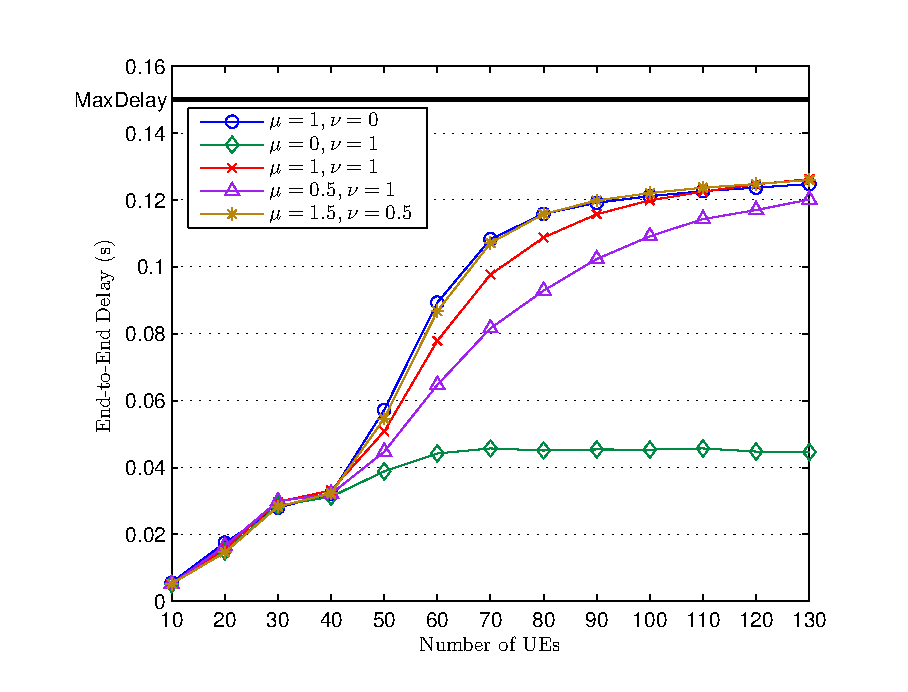
\includegraphics[%
  	scale=0.7,keepaspectratio]{figure/UFS/fixed/Delay_Video}
}
\subfigure[\label{fig:UFS_ran_delay_video}隨機服務流數量下UFS使用不同指數時Video的端點對端點延遲。]{
	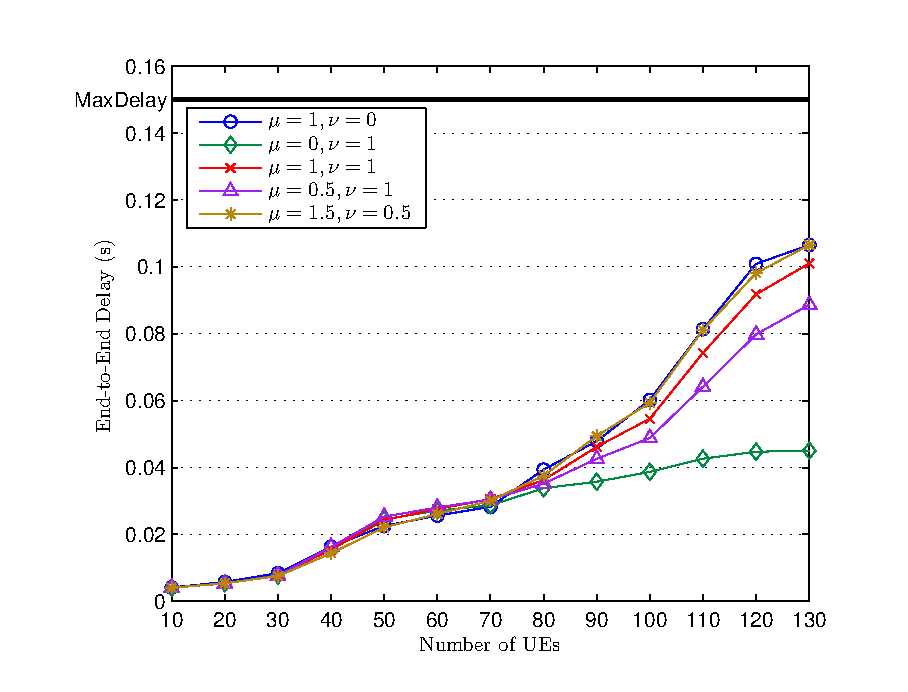
\includegraphics[%
	scale=0.7,keepaspectratio]{figure/UFS/random/Delay_Video}
}
\caption{\label{fig:UFS_delay_video}不同環境中UFS使用不同指數時Video服務流的端點對端點延遲。}
\end{figure}
\begin{figure}[H]
\centering
\subfigure[\label{fig:UFS_fix_delay_web}固定服務流數量下UFS使用不同指數時Web的端點對端點延遲。]{
 	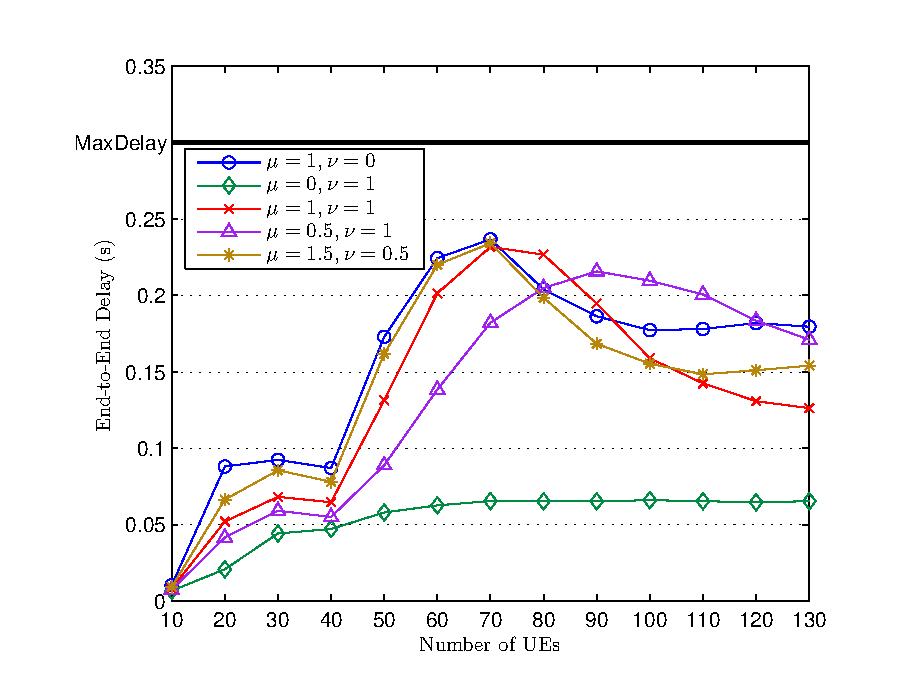
\includegraphics[%
  	scale=0.7,keepaspectratio]{figure/UFS/fixed/Delay_Web}
}
\subfigure[\label{fig:UFS_ran_delay_web}隨機服務流數量下UFS使用不同指數時Web的端點對端點延遲。]{
 	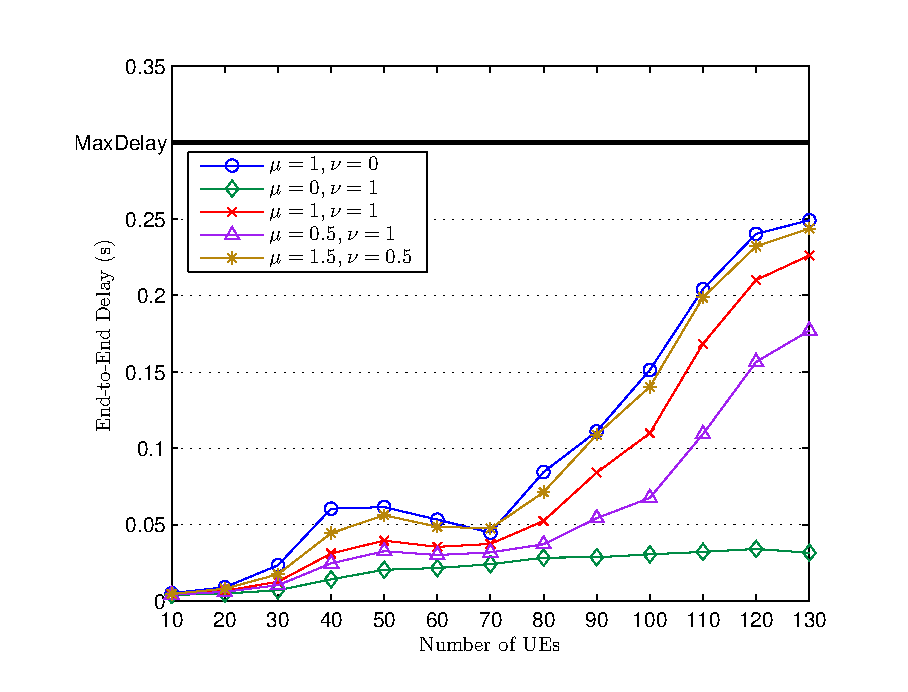
\includegraphics[%
  	scale=0.7,keepaspectratio]{figure/UFS/random/Delay_Web}
}
\caption{\label{fig:UFS_delay_web}不同環境中UFS使用不同指數時Web服務流的端點對端點延遲。}
\end{figure}
圖 \ref{fig:UFS_delay_voip}、圖 \ref{fig:UFS_delay_video}、圖 \ref{fig:UFS_delay_web}分別為不同環境下UFS使用不同指數時對各服務流的端點對端點延遲影響,可以發現當$\mu=1,\nu=0$時會有最高的端點對端點延遲,原因在於此時使用者裝置取得資源的優先順序完全由急迫度$U_i(t)$控制,使用者裝置只有在服務流延遲預算剩餘時間越來越少時才有機會優先取得資源,因此,封包在佇列中的延遲時間便會增加;當$\mu=0,\nu=1$時,各服務流的端點對端點延遲時間都會是最低的,此時使用者裝置取得資源的優先順序則是由平均配置資源度$\overline{A_i(t)}$決定,封包在佇列中的延遲預算剩餘時間不影響優先權值$P_i(t)$,因此,在使用者裝置佇列中的封包不會被迫等待至接近延遲預算上限才得到資源,各服務流佇列中的封包延遲時間減少。
\begin{figure}[H]
\centering
\subfigure[\label{fig:UFS_fix_PLR}固定服務流數量下UFS使用不同指數時的封包遺失率。]{
 	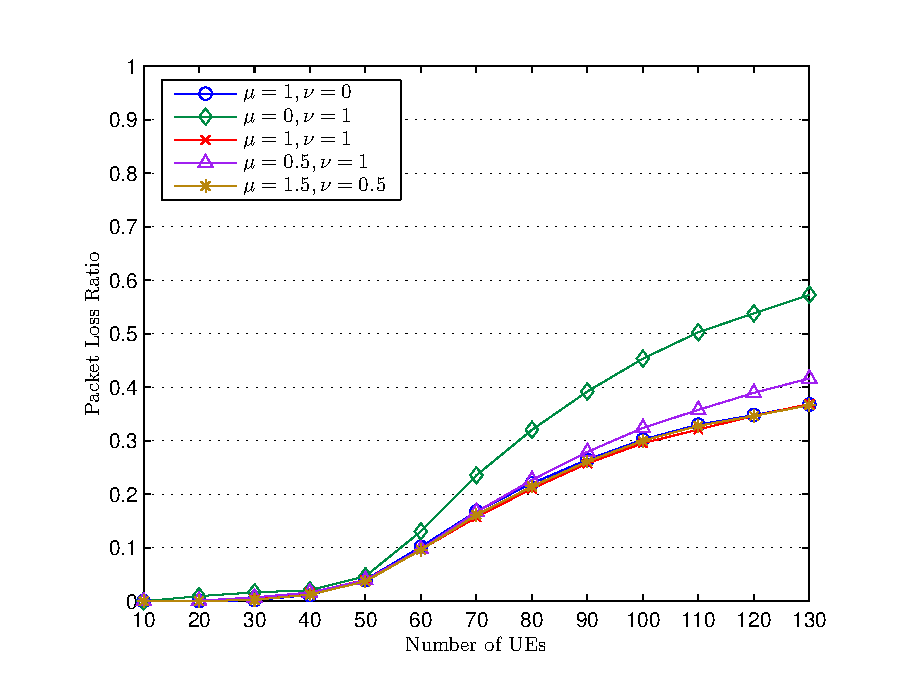
\includegraphics[%
  	scale=0.7,keepaspectratio]{figure/UFS/fixed/PLR}
}
\subfigure[\label{fig:UFS_ran_PLR}隨機服務流數量下UFS使用不同指數時的封包遺失率。]{
	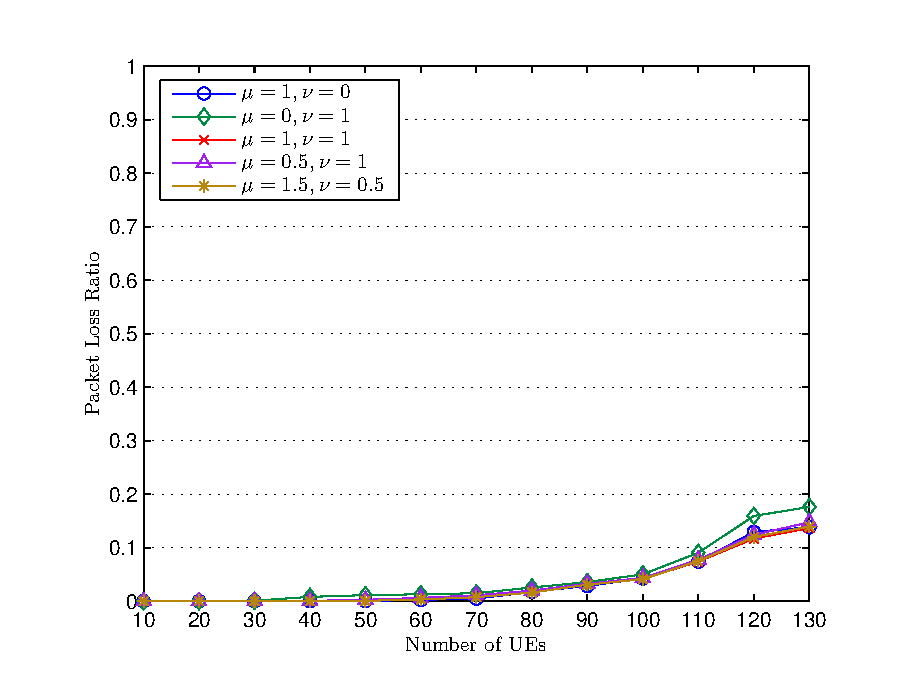
\includegraphics[%
	scale=0.7,keepaspectratio]{figure/UFS/random/PLR}
}
\caption{\label{fig:UFS_PLR}不同環境中UFS使用不同指數時的封包遺失率。}
\end{figure}
圖 \ref{fig:UFS_PLR}為不同環境下UFS使用不同指數時對封包遺失率的影響。當$\mu=0,\nu=1$時,在兩種不同環境都會有最高的封包遺失率,因為其並不考慮使用者裝置內佇列中封包的延遲情形,封包遺失率會高於其他$\mu > 0$考慮使用者裝置急迫度時的情況;當$\mu=0.5,\mu=1,\mu=1.5$時,不論是否$\nu>0$或是$\nu=0$,都能有較低的封包遺失率,同時,彼此之間的差距微小,因為考量了使用者裝置的急迫度,佇列中的封包在超過延遲預算之前使用者裝置便有機會取得資源,封包在佇列中超過延遲預算被丟棄的機率下降。
\begin{figure}[H]
\centering
\subfigure[\label{fig:UFS_fix_fairness}固定服務流數量下UFS使用不同指數時的公平性。]{
 	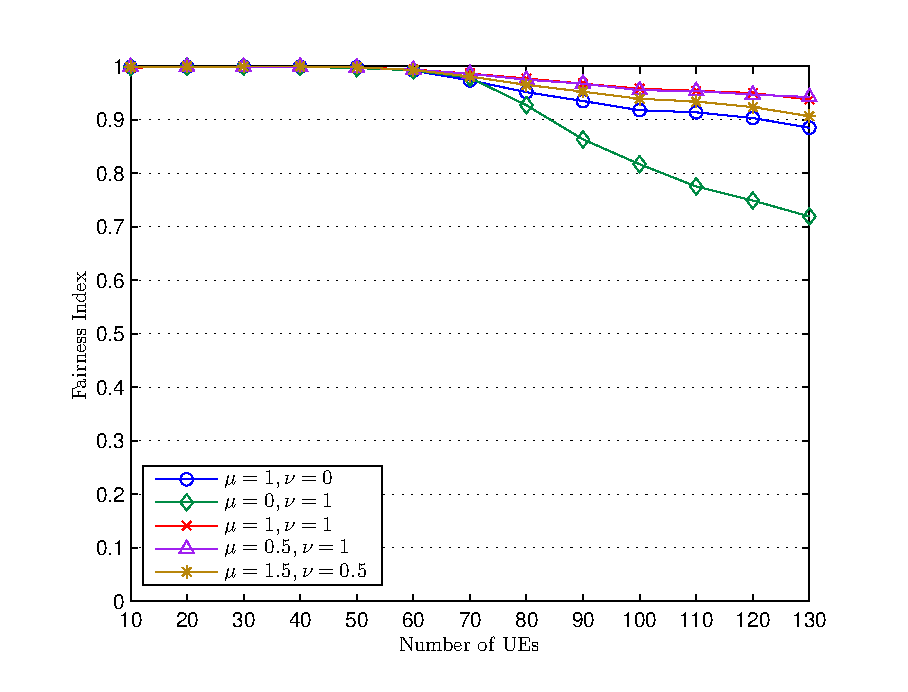
\includegraphics[%
  	scale=0.7,keepaspectratio]{figure/UFS/fixed/Fairness}
}
\subfigure[\label{fig:UFS_ran_fairness}隨機服務流數量下UFS使用不同指數時的公平性。]{
	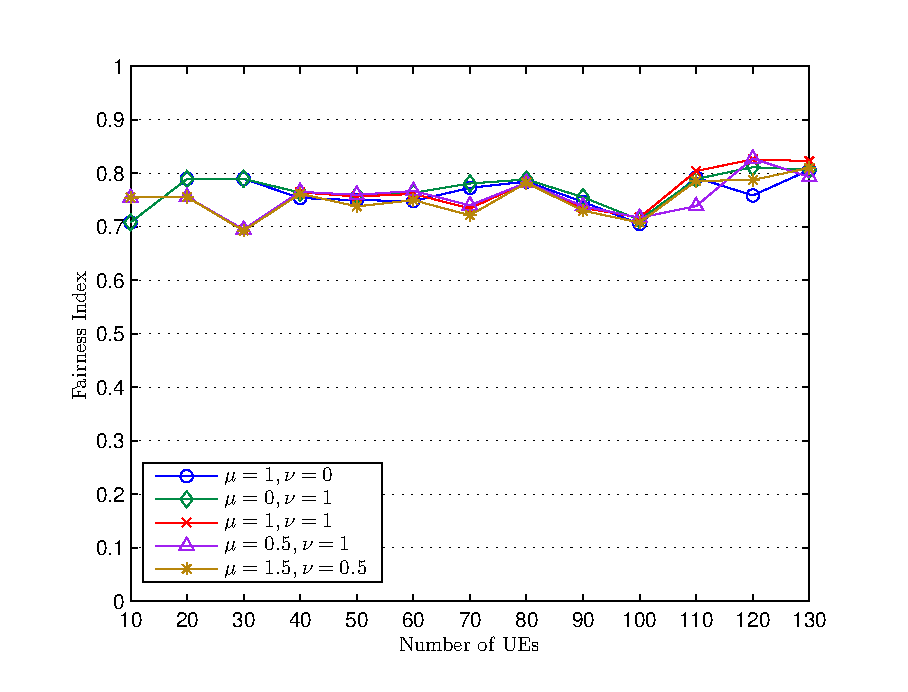
\includegraphics[%
	scale=0.7,keepaspectratio]{figure/UFS/random/Fairness}
}
\caption{\label{fig:UFS_Fairness}不同環境中UFS使用不同指數時的公平性。}
\end{figure}
圖 \ref{fig:UFS_Fairness}為不同環境下UFS使用不同指數時對公平性的影響。在圖 \ref{fig:UFS_fix_fairness}中,當$\mu=0,\nu=1$時整體的公平性最低,因為只以平均配置資源度決定使用者裝置取得資源的優先順序,較高的封包遺失率讓整體公平性下降;從$\mu=1,\nu=0$與$\mu=1,\nu=1$的結果可以發現,僅考量使用者裝置的急迫度時,整體的公平性已經有不錯的表現,但是,將平均配置資源度加入調整優先權值後,可以有更佳的整體公平性。
\begin{figure}[H]
\centering
\subfigure[\label{fig:UFS_fix_Throughput}固定服務流數量下UFS使用不同指數時的吞吐量。]{
 	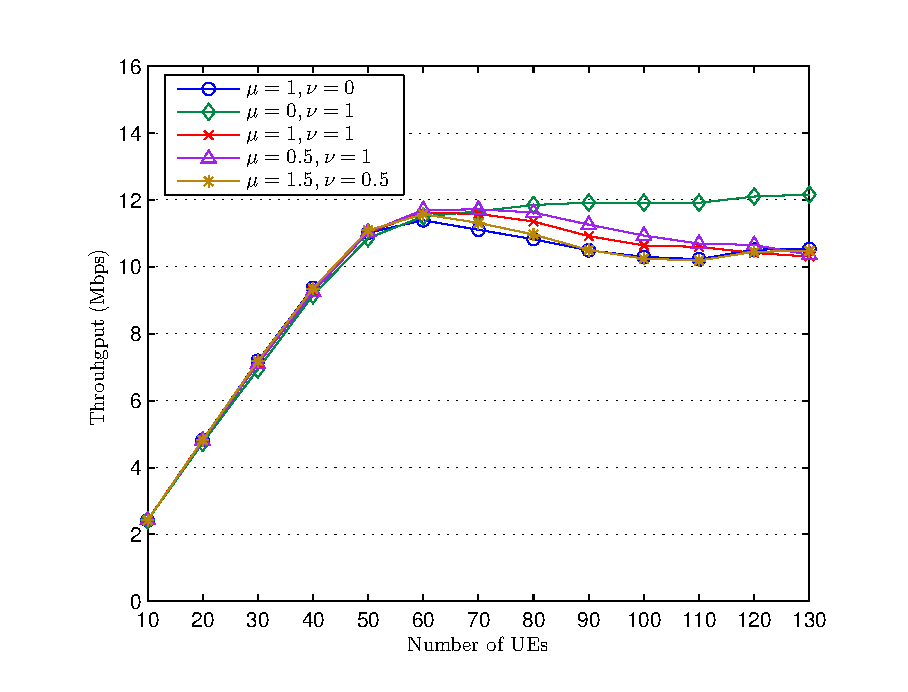
\includegraphics[%
  	scale=0.7,keepaspectratio]{figure/UFS/fixed/Throughput}
}
\subfigure[\label{fig:UFS_ran_Throughput}隨機服務流數量下UFS使用不同指數時的吞吐量。]{
	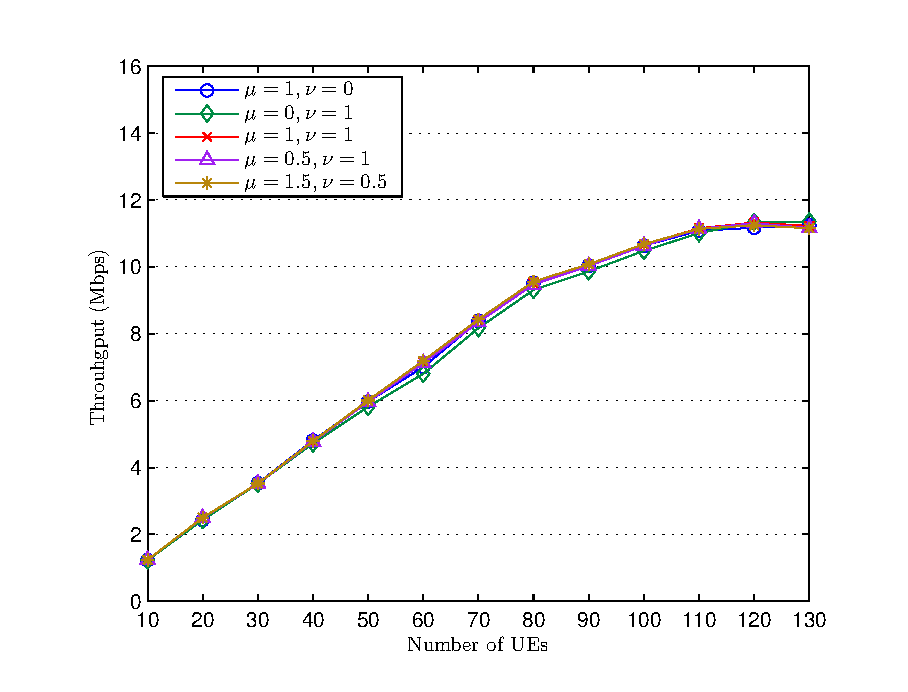
\includegraphics[%
	scale=0.7,keepaspectratio]{figure/UFS/random/Throughput}
}
\caption{\label{fig:UFS_Throughput}不同環境中UFS使用不同指數時的吞吐量。}
\end{figure}
圖 \ref{fig:UFS_Throughput}為不同環境下UFS使用不同指數時對吞吐量的影響。在圖 \ref{fig:UFS_fix_Throughput}中可以發現,當$\mu=0,\nu=1$時系統的吞吐量比其他情況都高,原因在於固定服務流數量時,使用者裝置中的服務流種類和數量固定,造成當$\mu>0$將使用者裝置急迫度加入優先權值的考量時,使用者裝置之間的急迫度差異不大,使UFS的循環性程度上升,整體的吞吐量下降;在隨機服務流數量時,使用者裝置之間的服務流種類與數量皆不盡相同,急迫度的差異性明顯,資源分配上可以得到更高的效果。

透過圖 \ref{fig:UFS_delay_voip}、圖 \ref{fig:UFS_delay_video}、圖 \ref{fig:UFS_delay_web}、圖 \ref{fig:UFS_PLR}、圖 \ref{fig:UFS_Fairness}、圖 \ref{fig:UFS_Throughput},我們可以發現,調整UFS中急迫度$U_i(t)$與平均配置資源度$\overline{A_i(t)}$的指數$\mu,\nu$,可以改變急迫度與平均配置資源度在不同評估結果上的影響。在$1 \leq \mu \leq \mu_{MAX}$的範圍中,當$\mu$越大時,急迫度對優先順序的影響程度上升,封包預算剩餘時間越短的使用者裝置即使配置過較多的資源區塊,仍然會比其他使用者裝置容易得到資源,可以減少封包在佇列中被丟棄的機率,降低整體的封包遺失率;在$0 \leq \nu \leq 1$的範圍中,當$\nu$越大時,平均配置資源度的影響上升,在端點對端點延遲上可以有較低的延遲。我們可以針對想要提升的特定效果,選擇不同的指數來調整急迫度與平均配置資源度對優先權值的影響;我們同時也可以發現,平均配置資源度對優先順序的影響程度並不如急迫度,主要用於輔助調整優先權值,同時,當$\mu=1,\nu=1$時,從各項較能評估結果綜合來看,可以取得較好的效果,因此,在本章節之後用於比較各方法之間的效能評估時,UFS皆使用$\mu=1,\nu=1$做為公式(\ref{Priority})中的指數數值,與其他方法在不同方面上的評估進行比較。

\subsection{調變編碼技術限制效果}
排程演算法在資源區塊的連續分配的方式上有各種不同的設計,一般的排程演算法利用通道品質決定連續分配的方式,而UFS則是使用調變編碼技術限制來決定分配給使用者裝置的資源區塊數量。UFS在資源連續分配的階段時,會依照公式(\ref{Threshold})判斷此次的排程是否使用調變編碼技術限制,滿足公式(\ref{Threshold})則會啟用限制並檢查分配該資源區塊是否會影響原先可以使用的調變編碼技術,若會造成原本可使用的調變等級下降,則不分配該資源區塊給使用者裝置,接著對下一個優先順序的使用者裝置開始分配資源。為能了解在資源區塊連續分配時使用調變編碼技術限制的影響,我們比較UFS在第一階段決定使用者裝置的分配資源優先順序後,於第二階段的資源區塊連續分配的方式上,使用調變編碼技術限制資源區塊數量(MCS-Constraint Sequential Allocation)以及分配固定資源區塊數量(Fixed Amount Sequential Allocation)兩種不同的連續分配方式,觀察在各服務流的端點對端點延遲、封包遺失率、公平性與吞吐量上的結果。
\begin{comment}
\begin{figure}[H]
\centering
\subfigure[\label{fig:MCS_fix_delay}固定服務流數量使用不同連續分配方式時的整體端點對端點延遲。]{
 	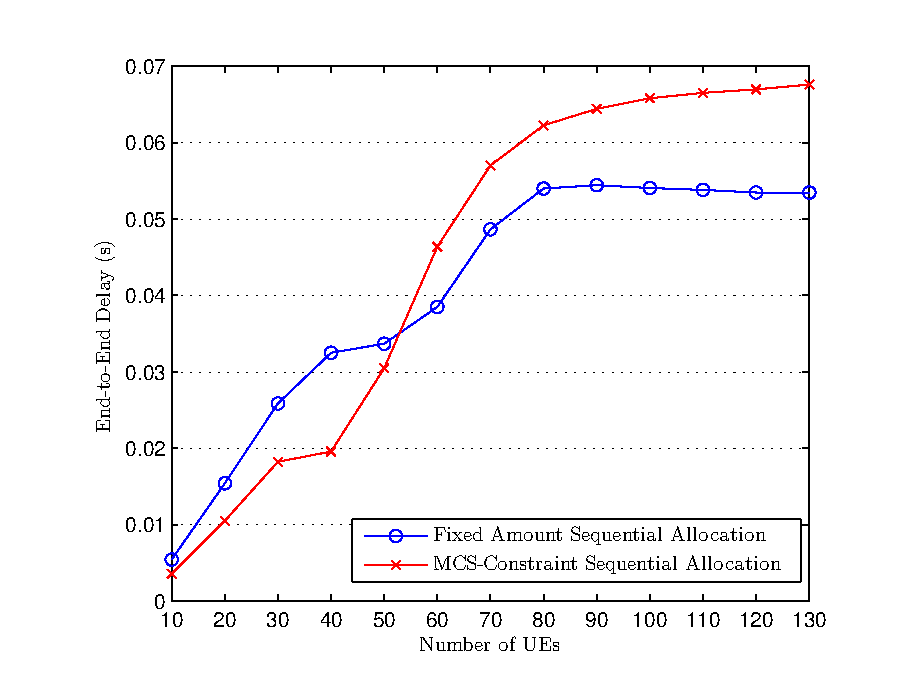
\includegraphics[%
  	scale=0.7,keepaspectratio]{figure/MCS/fixed/Delay}
}
\subfigure[\label{fig:MCS_ran_delay}隨機服務流數量使用不同連續分配方式時的整體端點對端點延遲。]{
	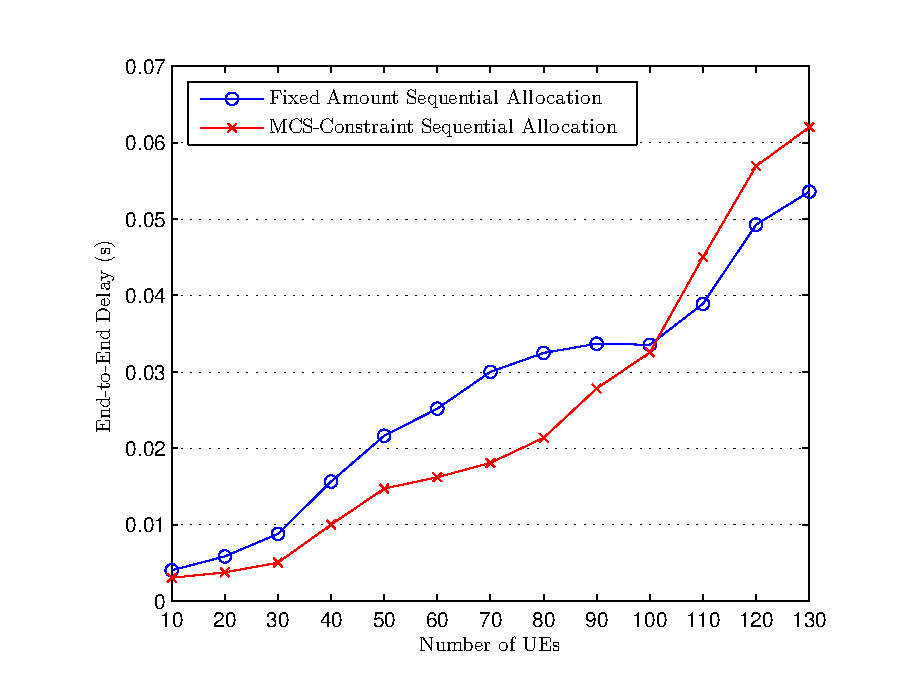
\includegraphics[%
	scale=0.7,keepaspectratio]{figure/MCS/random/Delay}
}
\caption{\label{fig:MCS_delay}不同環境中UFS使用不同連續分配方式時的端點對端點延遲。}
\end{figure}
\end{comment}
\begin{figure}[H]
\centering
\subfigure[\label{fig:MCS_fix_delay_voip}固定服務流數量下使用不同連續分配方式時VoIP的端點對端點延遲。]{
 	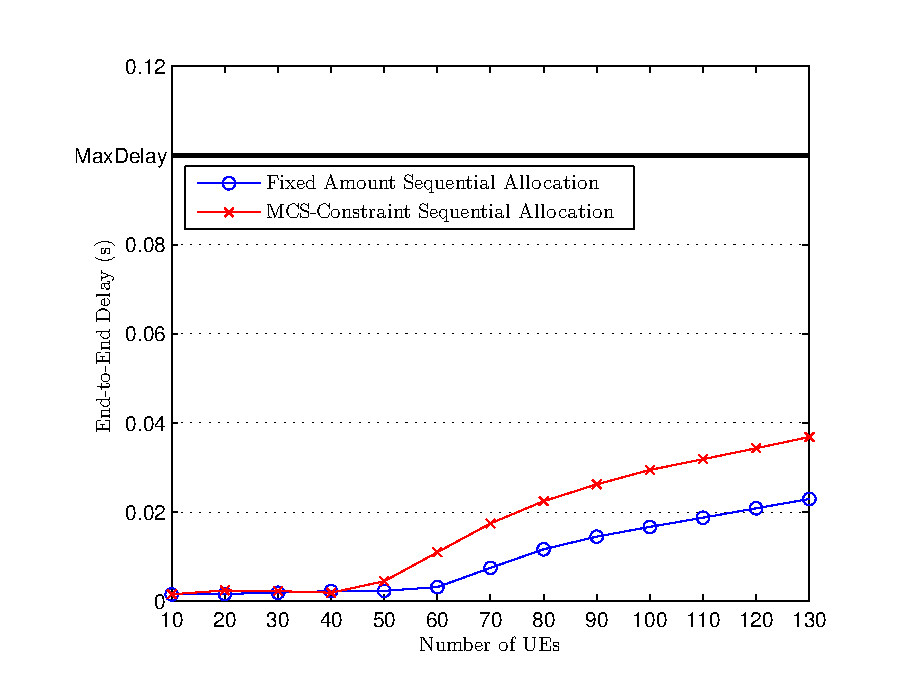
\includegraphics[%
  	scale=0.7,keepaspectratio]{figure/MCS/fixed/Delay_VoIP}
}
\subfigure[\label{fig:MCS_ran_delay_voip}隨機服務流數量下使用不同連續分配方式時VoIP的端點對端點延遲。]{
	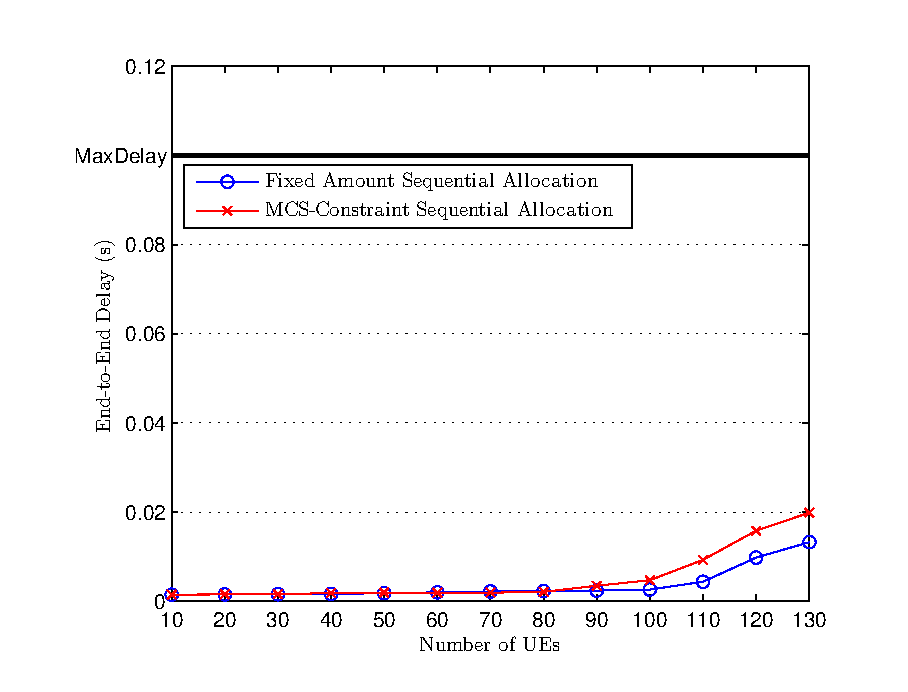
\includegraphics[%
	scale=0.7,keepaspectratio]{figure/MCS/random/Delay_VoIP}
}
\caption{\label{fig:MCS_delay_voip}不同環境中UFS使用不同連續分配方式時VoIP服務流的端點對端點延遲。}
\end{figure}
\begin{figure}[H]
\centering
\subfigure[\label{fig:MCS_fix_delay_video}固定服務流數量下使用不同連續分配方式時Video的端點對端點延遲。]{
 	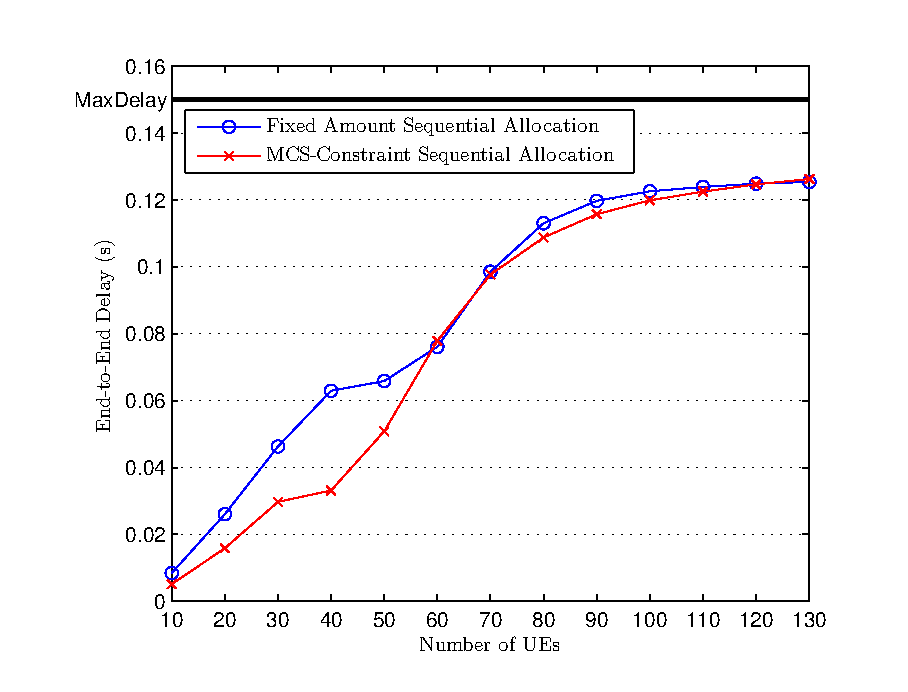
\includegraphics[%
  	scale=0.7,keepaspectratio]{figure/MCS/fixed/Delay_Video}
}
\subfigure[\label{fig:MCS_ran_delay_video}隨機服務流數量下使用不同連續分配方式時Video的端點對端點延遲。]{
	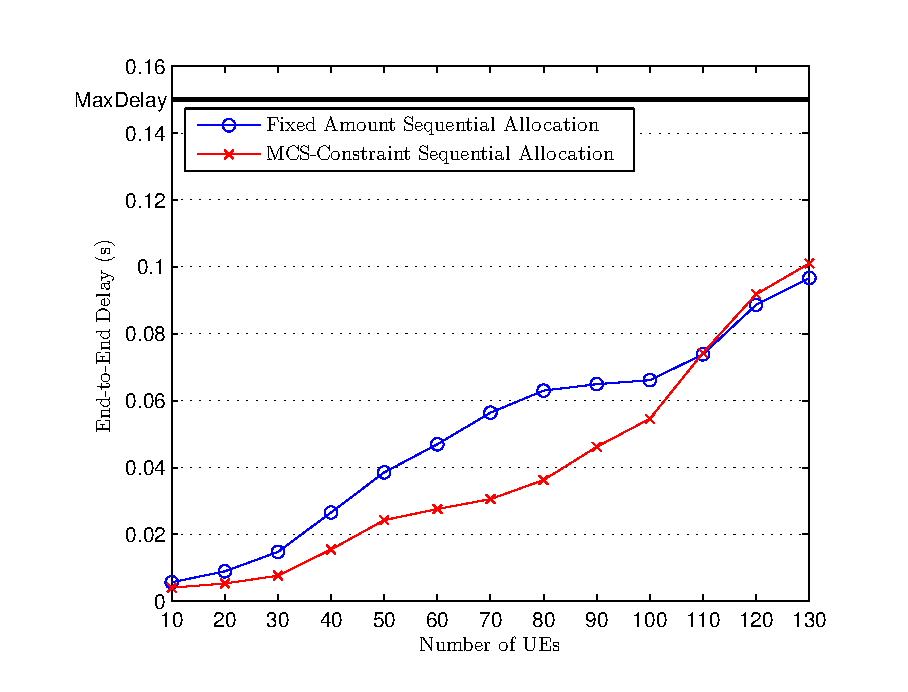
\includegraphics[%
	scale=0.7,keepaspectratio]{figure/MCS/random/Delay_Video}
}
\caption{\label{fig:MCS_delay_video}不同環境中UFS使用不同連續分配方式時Video服務流的端點對端點延遲。}
\end{figure}
\begin{figure}[H]
\centering
\subfigure[\label{fig:MCS_fix_delay_web}固定服務流數量下使用不同連續分配方式時Web的端點對端點延遲。]{
 	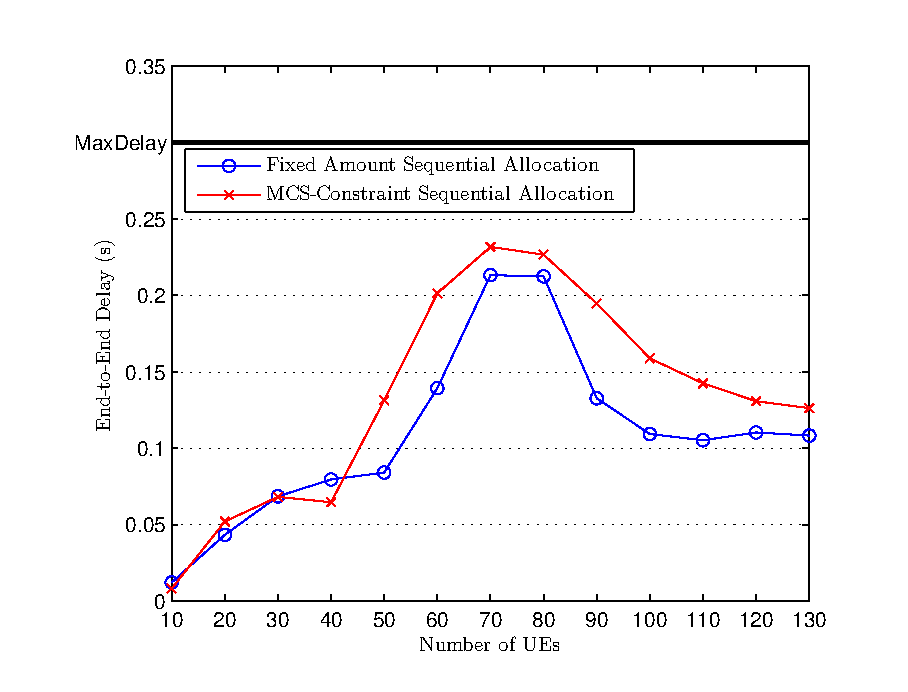
\includegraphics[%
  	scale=0.7,keepaspectratio]{figure/MCS/fixed/Delay_Web}
}
\subfigure[\label{fig:MCS_ran_delay_web}隨機服務流數量下使用不同連續分配方式時Web的端點對端點延遲。]{
 	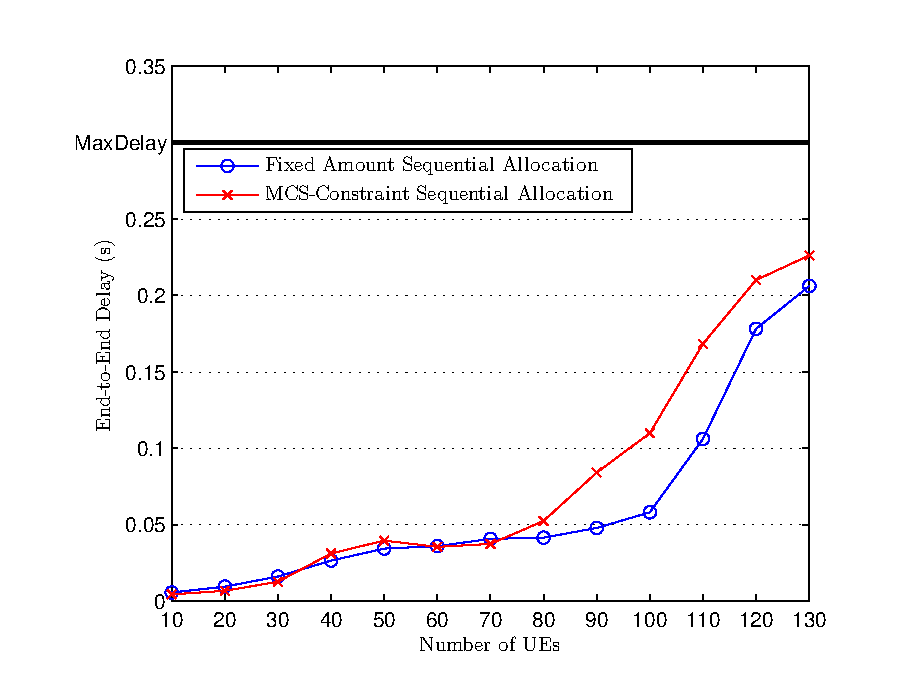
\includegraphics[%
  	scale=0.7,keepaspectratio]{figure/MCS/random/Delay_Web}
}
\caption{\label{fig:MCS_delay_web}不同環境中UFS使用不同連續分配方式時Web服務流的端點對端點延遲。}
\end{figure}
圖 \ref{fig:MCS_delay_voip}、圖 \ref{fig:MCS_delay_video}、圖 \ref{fig:MCS_delay_web}分別為使用不同的連續分配方式對各服務流的端點對端點延遲影響。我們可以發現使用調變編碼技術限制的連續分配方式在VoIP服務流會明顯有較高的延遲,Video服務流與Web服務流在較多使用者裝置時的延遲也會高於固定數量的連續分配方式,主要因為使用調變編碼技術限制時,排程器為了資源區塊能使用較高等級的調變技術,會限制使用者裝置可以取得的資源區塊數量,使用者裝置可能無法取得足夠的資源區塊傳輸佇列中的資料,使得封包在佇列中的等待時間變長,端點對端點延遲同時跟著增加;固定數量的連續分配方式在每次分配資源時會先根據使用者裝置的數量與可使用的資源區塊數量,決定平均一個使用者裝置可以取得的資源區塊數量,再依據優先順序依序分配連續的資源區塊給使用者裝置,因此,相較於使用調變編碼技術限制的連續分配方式,在單次的排程中使用者裝置可以取得較多資源區塊,可以傳輸佇列中的資料,減少封包在佇列中的延遲時間。

\begin{figure}[H]
\centering
\subfigure[\label{fig:MCS_fix_PLR}固定服務流數量下使用不同連續分配方式時的封包遺失率。]{
 	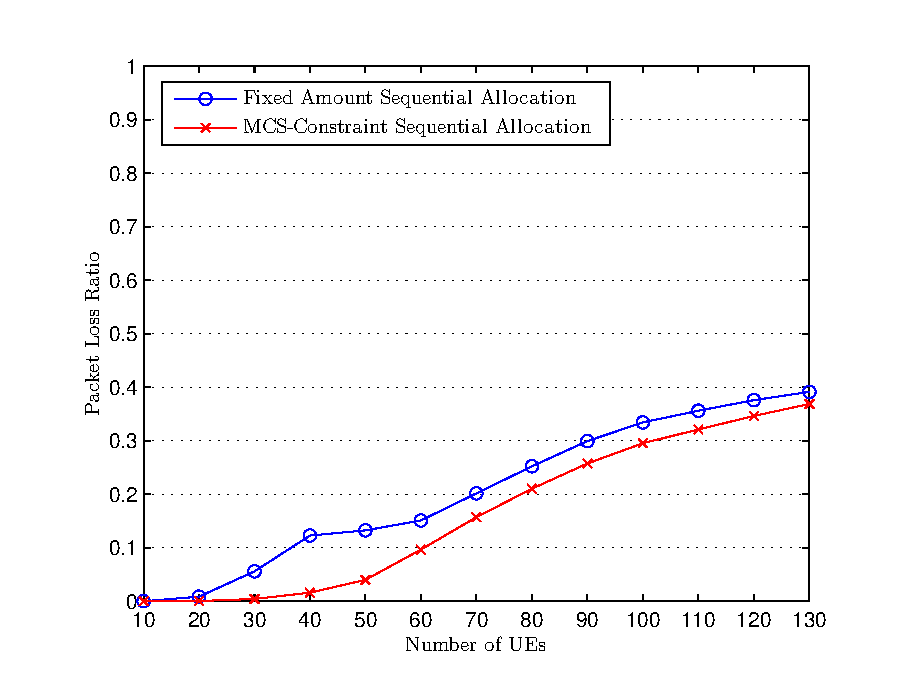
\includegraphics[%
  	scale=0.7,keepaspectratio]{figure/MCS/fixed/PLR}
}
\subfigure[\label{fig:MCS_ran_PLR}隨機服務流數量下使用不同連續分配方式時的封包遺失率。]{
	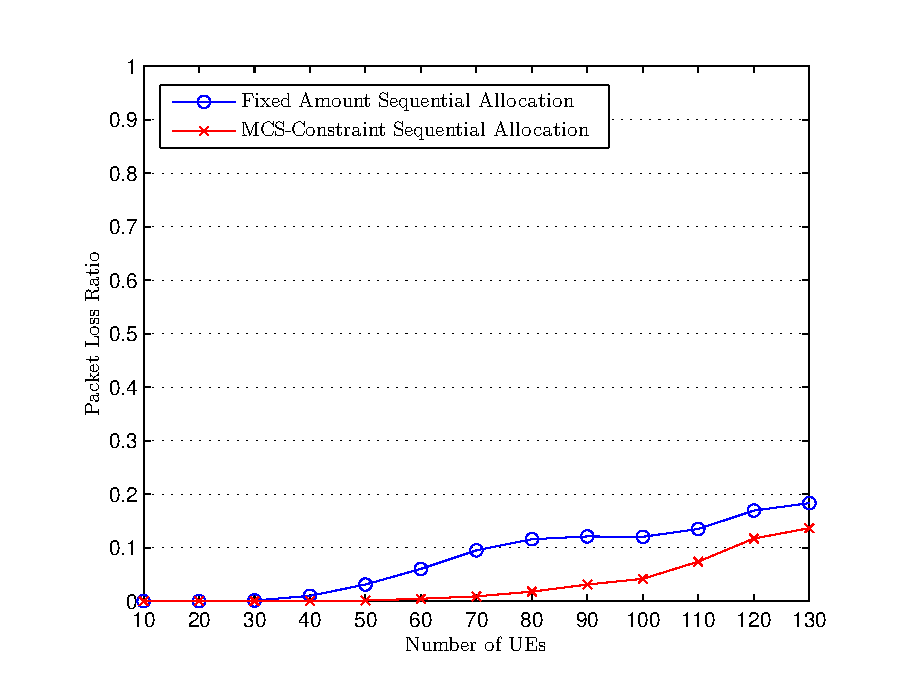
\includegraphics[%
	scale=0.7,keepaspectratio]{figure/MCS/random/PLR}
}
\caption{\label{fig:MCS_PLR}不同環境中UFS使用不同連續分配方式時的封包遺失率。}
\end{figure}
\begin{figure}[H]
\centering
\subfigure[\label{fig:MCS_fix_fairness}固定服務流數量下使用不同連續分配方式時的公平性。]{
 	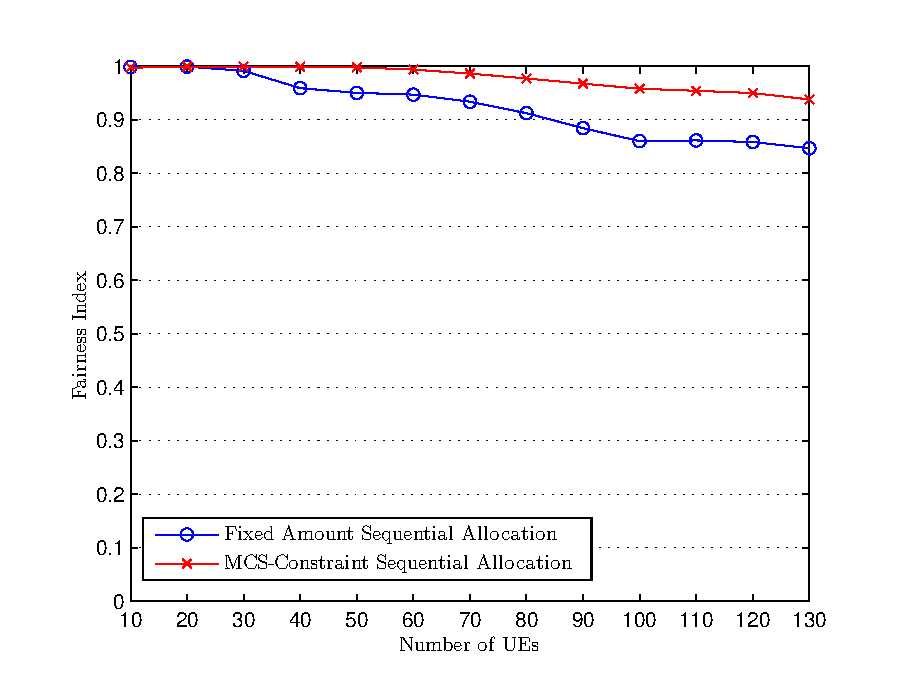
\includegraphics[%
  	scale=0.7,keepaspectratio]{figure/MCS/fixed/Fairness}
}
\subfigure[\label{fig:MCS_ran_fairness}隨機服務流數量下使用不同連續分配方式時的公平性。]{
	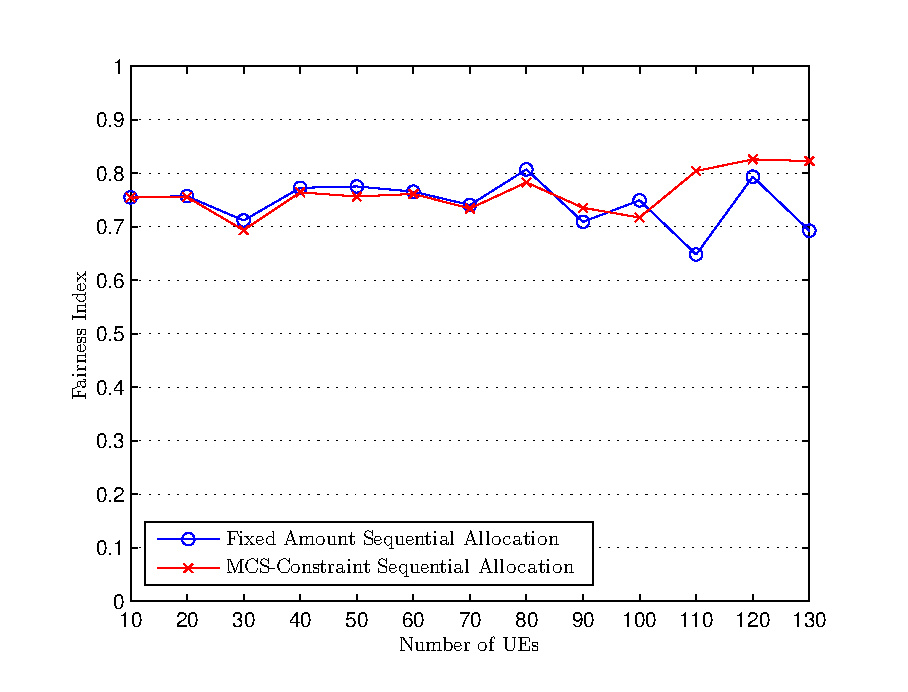
\includegraphics[%
	scale=0.7,keepaspectratio]{figure/MCS/random/Fairness}
}
\caption{\label{fig:MCS_Fairness}不同環境中UFS使用不同連續分配方式時的公平性。}
\end{figure}
\begin{figure}[H]
\centering
\subfigure[\label{fig:MCS_fix_Throughput}固定服務流數量下使用不同連續分配方式時的吞吐量。]{
 	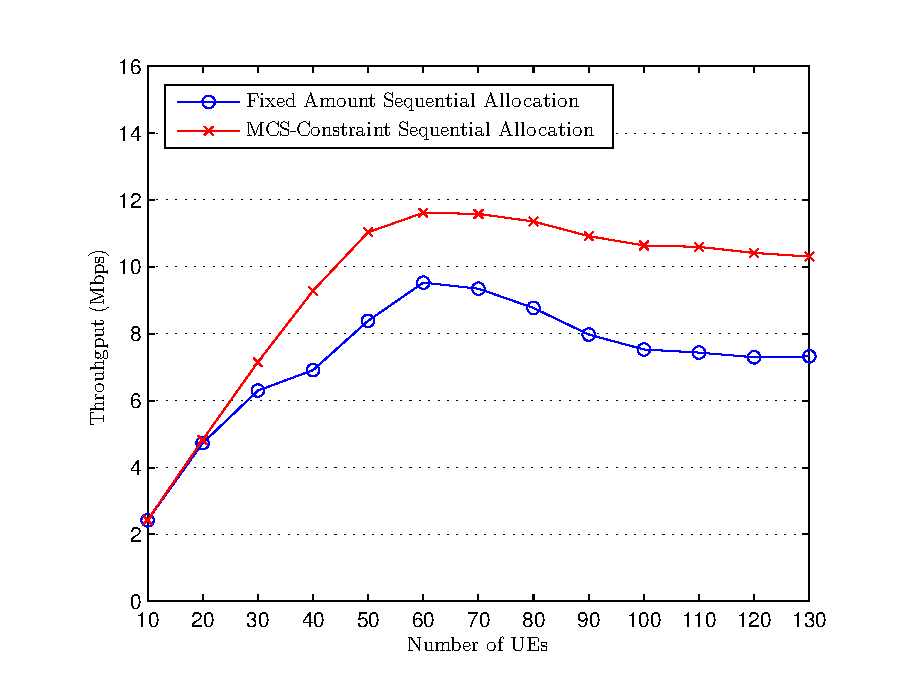
\includegraphics[%
  	scale=0.7,keepaspectratio]{figure/MCS/fixed/Throughput}
}
\subfigure[\label{fig:MCS_ran_Throughput}隨機服務流數量下使用不同連續分配方式時的吞吐量。]{
	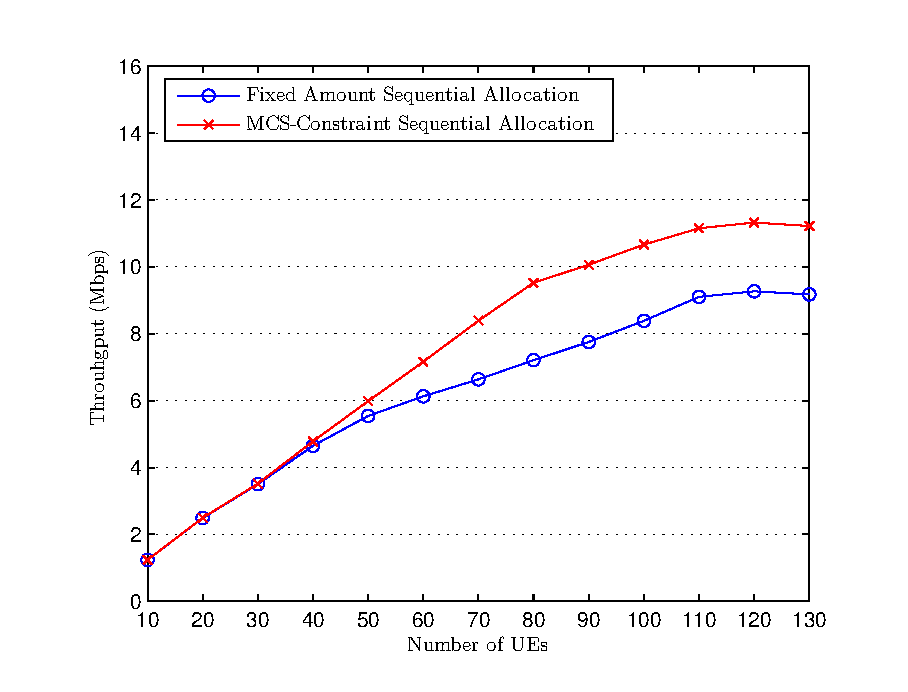
\includegraphics[%
	scale=0.7,keepaspectratio]{figure/MCS/random/Throughput}
}
\caption{\label{fig:MCS_Throughput}不同環境中UFS使用不同連續分配方式時的吞吐量。}
\end{figure}
圖 \ref{fig:MCS_PLR}、圖 \ref{fig:MCS_Fairness}、圖 \ref{fig:MCS_Throughput}分別為使用不同的連續分配方式對整體的封包遺失率、公平性與吞吐量的影響。在資源區塊的連續分配上使用調變編碼技術限制時,這三種結果上都可以比固定數量的連續分配方式有更好的效果,主要原因在於,雖然調變編碼技術限制有機率會讓使用者裝置可以取得的資源區塊數量下降,但是,在單次的排程時會有更多使用者裝置可以取得資源區塊傳輸在佇列中等待的封包,降低封包遺失率以及提升使用者裝置之間的公平性;同時,調變編碼技術限制最主要的目的在維持資源區塊能使用的調變技術等級,提升資源區塊的資料傳輸效率,讓整體的吞吐量上升。綜合上述對連續分配方式的討論,在資源區塊的連續分配上使用調變編碼技術限制時,雖然在較多使用者裝置的環境時比固定數量的連續分配方式有更高的端點對端點延遲,但是,在封包遺失率、公平性與吞吐量上都會有較好的效果。

\section{各機制之端點對端點延遲}
端點對端點延遲為封包在佇列中的等待時間加上傳輸時間所得到的延遲時間,端點對端點延遲數值越高,表示封包從進入使用者裝置中的媒體存取控制層佇列開始,到抵達基地台中間的這段時間越長,對延遲敏感的服務流造成的影響越大;反之,端點對端點延遲數值越低,則延遲敏感的服務流能提供較佳的服務品質。我們所提出的UFS將使用者裝置內服務流的平均延遲預算剩餘時間定義為急迫度,並將其加入排程演算法,做為分配資源時決策使用者裝置優先程度的依據之一,目的在於拯救佇列頭端封包即將因為延遲預算耗盡而被丟棄的使用者裝置,優先給予該使用者裝置資源去傳送佇列中的資料,因此,平均延遲預算剩餘時間越長的使用者裝置,會將資源優先讓給急迫度較高的使用者裝置,而自己被迫等待至自身平均的服務流佇列頭端封包剩餘時間小於其他人時,再取得資源來傳輸佇列中的資料,所以,UFS中使用者裝置內各服務流的延遲時間都會受到排程演算法中急迫度的影響,而向各自服務流的延遲預算逼近。

圖 \ref{fig:delay_voip}、圖 \ref{fig:delay_video}、圖 \ref{fig:delay_web}分別代表了在VoIP、Video、Web服務流在兩種服務流數量環境下的端點對端點延遲,從圖 \ref{fig:delay_voip}、圖 \ref{fig:delay_video}、圖 \ref{fig:delay_web}中可以發現,雖然UFS在VoIP、Video、Web三種服務流的延遲時間與BestCQI\cite{su2016}、RR\cite{arsh2015}、FME\cite{fmerme2008}、RME\cite{safa2012}、PF\cite{kush2002}、ODM\cite{kana2015}相比都擁有較高的延遲時間,但是在服務流VoIP、Video、Web的延遲時間都有分別保持在各自的的延遲預算0.1 s、0.15 s、0.3 s以下,超過各自服務流延遲預算上限的封包將會在佇列中被丟棄。在圖 \ref{fig:fix_delay_voip}中,固定服務流數量時,UFS下服務流VoIP的端點對端點延遲從使用者裝置數量為40時開始上升,並在使用者裝置數量達到70時高於其他排程演算法。當使用者裝置數量為130時,UFS下服務流VoIP的端點對端點延遲分別比RR、PF、RME、ODM、FME、BestCQI高出394\%、316\%、269\%、239\%、201\%、198\%,實際上的端點對端點延遲分別高出29.4 ms、28.0 ms、27.5 ms、26.9 ms、24.6 ms、24.5 ms,UFS的端點對端點延遲與其他排程演算法在實際的時間上差距並不大,而且距離延遲預算上限仍有一段時間。

在圖 \ref{fig:ran_delay_voip}中,在隨機服務流時,UFS下服務流VoIP的端點對端點延遲從使用者裝置數量為90時開始高於RME、PF與ODM,並在使用者裝置數量為120時高於其他排程演算法。當使用者裝置數量為130時,UFS下服務流VoIP的端點對端點延遲分別比ODM、PF、RME、RR、BestCQI、FME高出595\%、576\%、267\%、264\%、75\%、70\%,實際上的端點對端點延遲分別高出17.0 ms、16.9 ms、14.5 ms、14.4 ms、8.5 ms、8.2 ms,同樣在實際的時間上差距不大。從圖 \ref{fig:delay_voip}中可以發現,UFS在隨機服務流數量時端點對端點延遲時間會低於固定服務流數量,原因在於隨機服務流數量下時,使用者裝置中存在的服務流種類並不一致,使用者裝置之間的急迫度差異明顯,使用者裝置中存在VoIP服務流時容易比其他使用者裝置有著更低的平均延遲預算剩餘時間,亦即容易有著更高的急迫度,而更容易優先取得資源;在固定服務流時,使用者裝置內都存在相同種類及數量的服務流,因此,在UFS中使用者裝置之間的急迫度差異不明顯。
\begin{figure}[H]
\centering
\subfigure[\label{fig:fix_delay_voip}固定服務流數量下VoIP的端點對端點延遲。]{
 	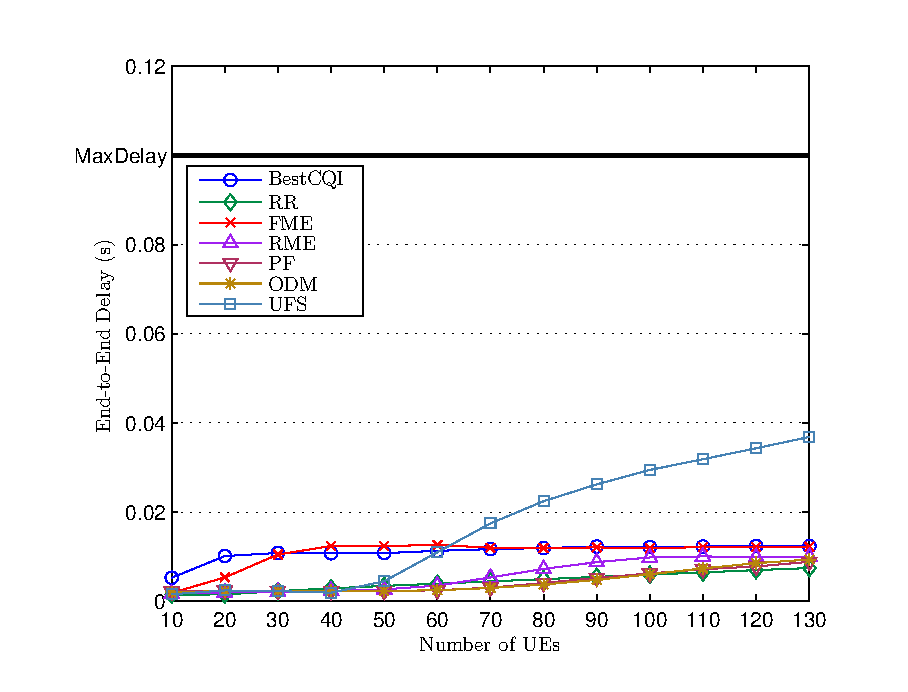
\includegraphics[%
  	scale=0.7,keepaspectratio]{figure/fixed/Delay_VoIP}
}
\subfigure[\label{fig:ran_delay_voip}隨機服務流數量下VoIP的端點對端點延遲。]{
	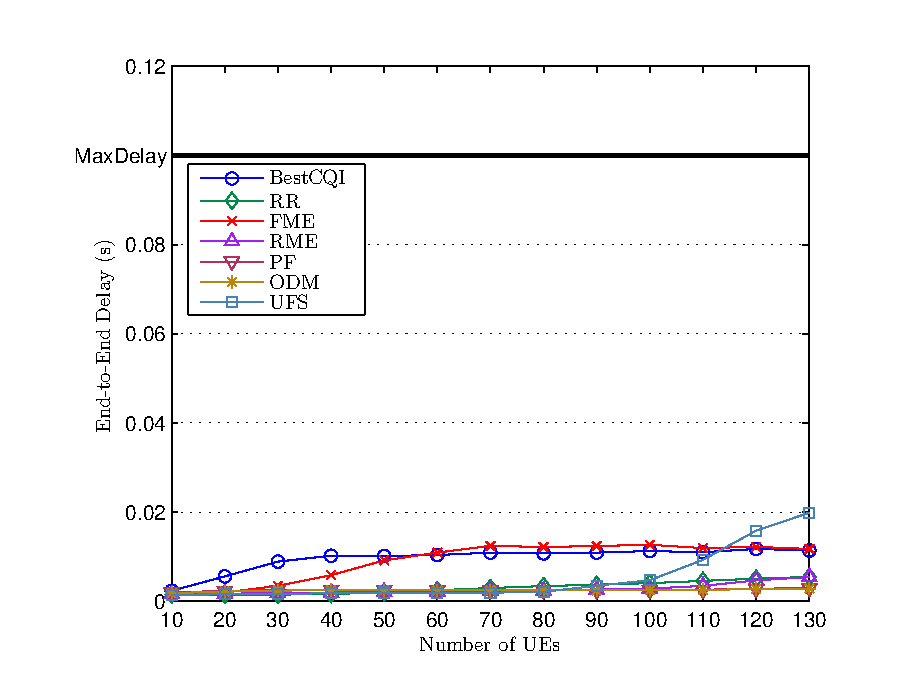
\includegraphics[%
	scale=0.7,keepaspectratio]{figure/random/Delay_VoIP}
}
\caption{\label{fig:delay_voip}不同環境中VoIP服務流的端點對端點延遲。}
\end{figure}
\clearpage
由圖 \ref{fig:fix_delay_video}可發現,固定服務流數量時,UFS下服務流Video的端點對端點延遲從使用者裝置數量為30時開始高於BestCQI並與FME相同,並在使用者裝置數量達到90時高於其他排程演算法。當使用者裝置數量為130時,UFS下服務流Video的端點對端點延遲分別比BestCQI、FME、RME、ODM、PF、RR高出610\%、393\%、140\%、59\%、42\%、7\%,UFS的端點對端點延遲除了RR之外,與其他排程演算法差距較大的原因在於將使用者裝置的平均延遲預算剩餘時間加入考量,因此,整體的端點對端點延遲會逼近延遲預算上限,不過仍保持在延遲預算上限之下;由圖 \ref{fig:ran_delay_video}中可發現,在隨機服務流時,UFS下服務流Video的端點對端點延遲在各使用者裝置數量皆低於RR,而從使用者裝置數量為50時開始高於BestCQI,並在使用者裝置數量為110時高於RR以外的其他排程演算法。當使用者裝置數量為130時,UFS下服務流Video的端點對端點延遲分別比BestCQI、FME、RME、ODM、PF高出463\%、284\%、70\%、51\%、46\%,UFS的端點對端點延遲會高於RR以外的排程演算法,但仍會維持在延遲預算上限之下。除此之外,UFS在隨機服務流數量時,端點對端點延遲皆會低於RR,並不像圖 \ref{fig:fix_delay_video}中使用者裝置數量達到90之後開始高於RR,主要原因在於隨機服務流數量時,使用者裝置之間的急迫度差異明顯,UFS會優先分配資源給平均延遲預算剩餘時間更少的使用者裝置,因此,擁有如Video等較低延遲預算上限服務流的使用者裝置較容易取得資源,RR並不考量使用者裝置內的服務流種類,僅分配固定量的資源區塊給距離上次分配最久的使用者裝置,因此,UFS的Video服務流端點對端點延遲會低於RR的Video服務流端點對端點延遲。
\begin{figure}[H]
\centering
\subfigure[\label{fig:fix_delay_video}固定服務流數量下Video的端點對端點延遲。]{
 	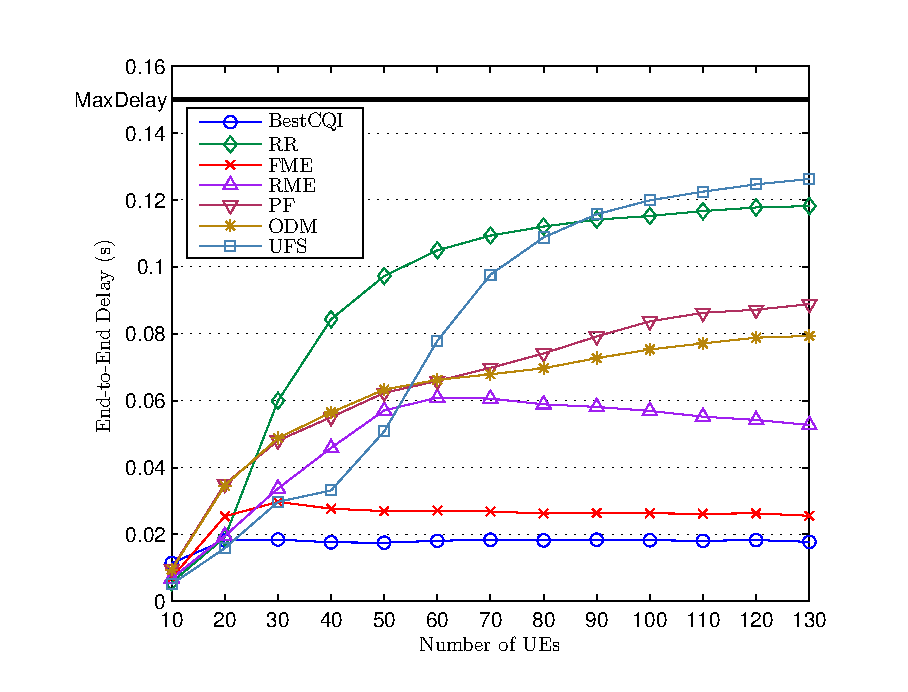
\includegraphics[%
  	scale=0.7,keepaspectratio]{figure/fixed/Delay_Video}
}
\subfigure[\label{fig:ran_delay_video}隨機服務流數量下Video的端點對端點延遲。]{
	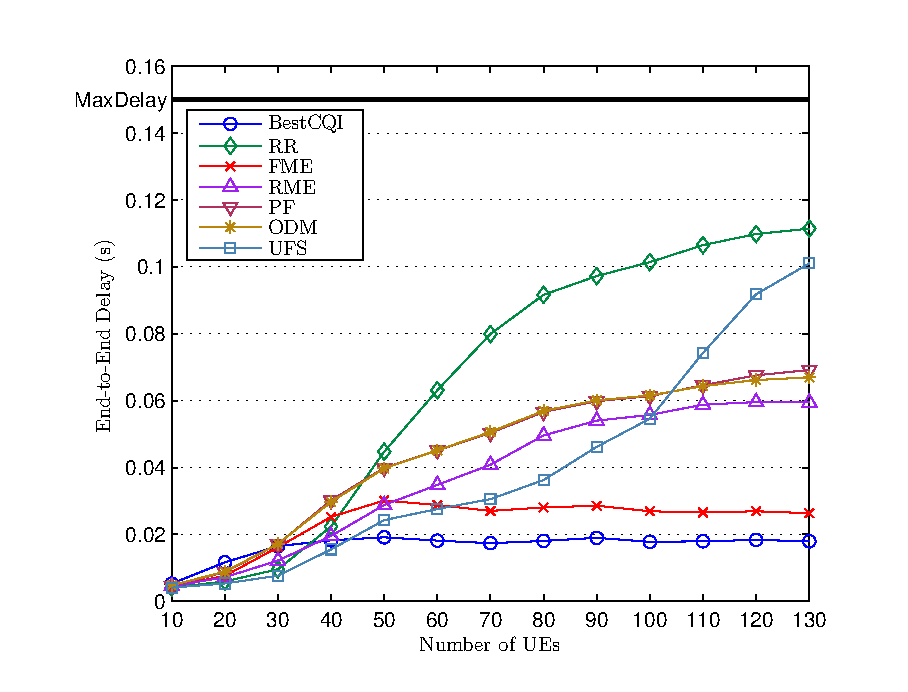
\includegraphics[%
	scale=0.7,keepaspectratio]{figure/random/Delay_Video}
}
\caption{\label{fig:delay_video}不同環境中Video服務流的端點對端點延遲。}
\end{figure}
\clearpage
由圖 \ref{fig:fix_delay_web}可發現,固定服務流數量時,UFS下服務流Web的端點對端點延遲受到分配量門檻值$\mathcal{A}_T$的影響,以使用者裝置數量為70時為分界,在使用者裝置數量小於70時,分配量$\mathcal{A}(t)$大於分配量門檻值的機率較高,啟動調變編碼技術限制的機率較小,使用者裝置一次可以取得足夠的資源進行傳輸,不過單次排程時分配到資源的使用者裝置也跟著下降,封包在佇列中等待的時間變長;從使用者裝置數量大於70開始,分配量$\mathcal{A}(t)$小於分配量門檻值的機率上升,啟動調變編碼技術限制的次數同時變多,使用者裝置一次可以取得的資源區塊數量下降,但是,同時增加單次排程時分配到資源的使用者裝置數量,有更多的Web資料流可以傳輸佇列中的資料,整體的端點對端點延遲下降。當使用者裝置數量為70時,UFS下服務流Web的端點對端點延遲分別比BestCQI、FME、ODM、RME、PF、RR高出825\%、642\%、356\%、273\%、169\%、104\%,實際上的端點對端點延遲分別高出206.8 ms、200.6 ms、181.0 ms、169.7.6 ms、145.6 ms、118.3 ms;由圖 \ref{fig:ran_delay_web}可發現,在隨機服務流時,UFS下服務流Web的端點對端點延遲從使用者裝置數量為80時高於其他排程演算法。當使用者裝置數量為130時,UFS下服務流Web的端點對端點延遲分別比BestCQI、ODM、FME、RME、PF、RR高出737\%、642\%、583\%、429\%、422\%、275\%,UFS的端點對端點延遲雖然會高於其他排程演算法,但仍會維持在延遲預算上限之下。除此之外,從圖 \ref{fig:delay_voip}、圖 \ref{fig:delay_video}、圖 \ref{fig:delay_web}中可以看出,BestCQI與FME的端點對端點延遲都維持在相當小的數值中,其主要原因在於這兩個排程演算法僅注重通道品質,且資源連續分配的方式容易造成該次排程只有少部分使用者裝置分配到資源,造成大量封包在佇列中被丟棄,而被丟棄的封包在佇列中的延遲時間並不被計算在端點對端點延遲中,因此,BestCQI與FME的端點對端點延遲會維持在較低的數值。關於封包遺失會在第4.4節中詳細敘述。
\begin{figure}[H]
\centering
\subfigure[\label{fig:fix_delay_web}固定服務流數量下Web的端點對端點延遲。]{
 	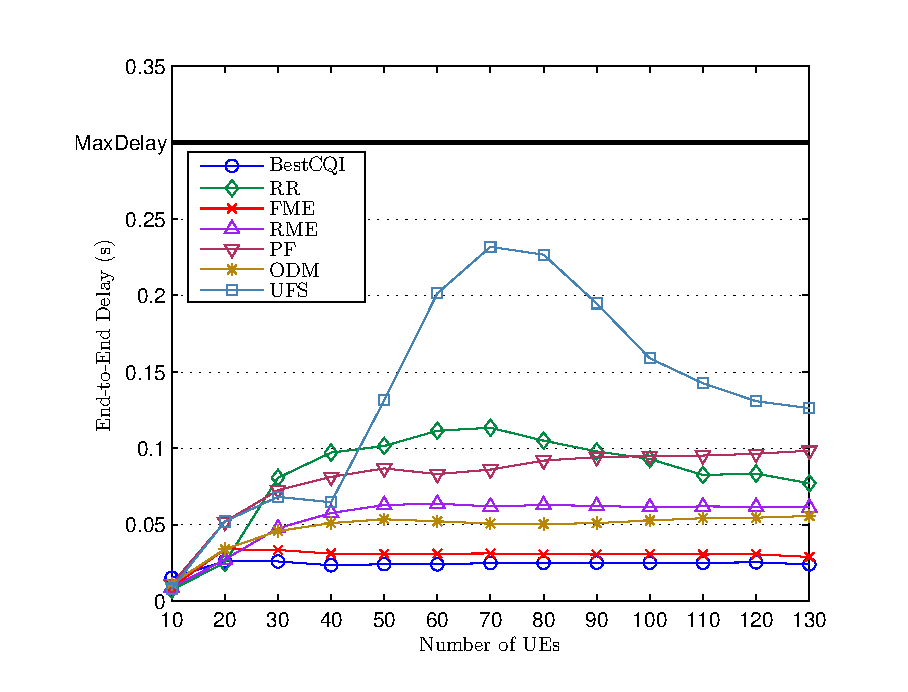
\includegraphics[%
  	scale=0.7,keepaspectratio]{figure/fixed/Delay_Web}
}
\subfigure[\label{fig:ran_delay_web}隨機服務流數量下Web的端點對端點延遲。]{
 	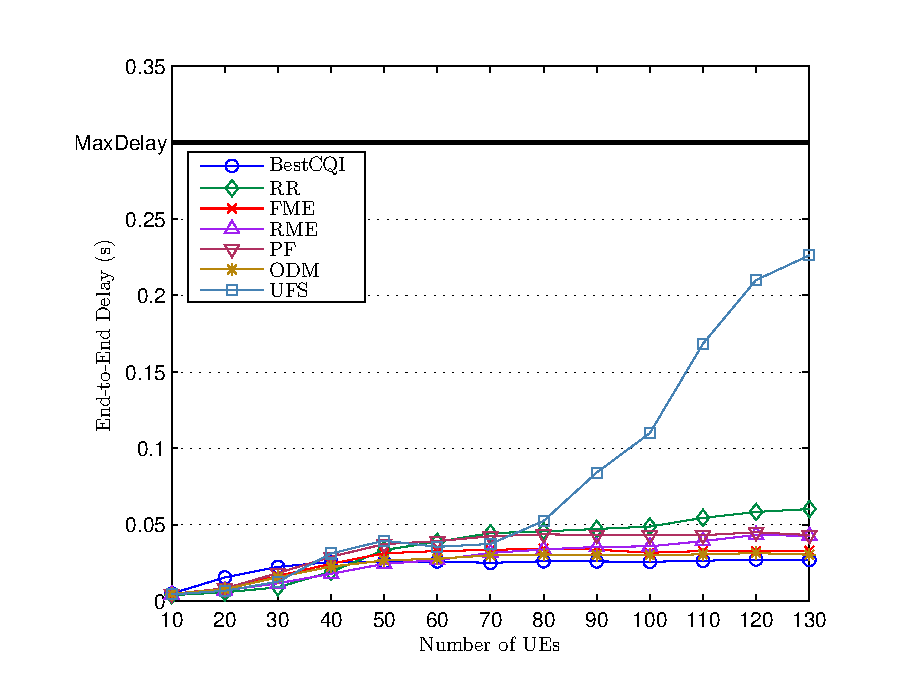
\includegraphics[%
  	scale=0.7,keepaspectratio]{figure/random/Delay_Web}
}
\caption{\label{fig:delay_web}不同環境中Web服務流的端點對端點延遲。}
\end{figure}
\begin{comment}%Delay table
\begin{table}[H]
\centering
\caption{不同服務流數量下端點對端點延遲時間差異幅度表。}
\vskip 10pt
\label{tab:delay_comp}
\begin{tabular}{|c|c|l|}
\hline
\multicolumn{1}{|l|}{} & \multicolumn{2}{c|}{UFS}              \\ \cline{2-3}
         & Fixed Flows      & \multicolumn{1}{c|}{Random Flows} \\ \hline
Best CQI & -59.02\% $\sim$ +342.76\% & -61.45\% $\sim$ +314.22\%  \\
RR       & -49.63\% $\sim$ +211.85\% & -52.32\% $\sim$ +95.13\%  \\
FME      & -35.00\% $\sim$ +258.29\% & -50.83\% $\sim$ +223.85\%  \\
RME      & -22.22\% $\sim$ +132.42\% & -32.31\% $\sim$ +108.15\%  \\
ODM      & -47.14\% $\sim$ +89.93\%  & -51.91\% $\sim$ +90.40\% \\ \hline
\end{tabular}
\end{table}
\end{comment}
\begin{comment}%Delay_All figure
\begin{figure}[H]
\centering
\subfigure[\label{fig:fix_delay}固定服務流數量下整體端點對端點延遲。]{
 	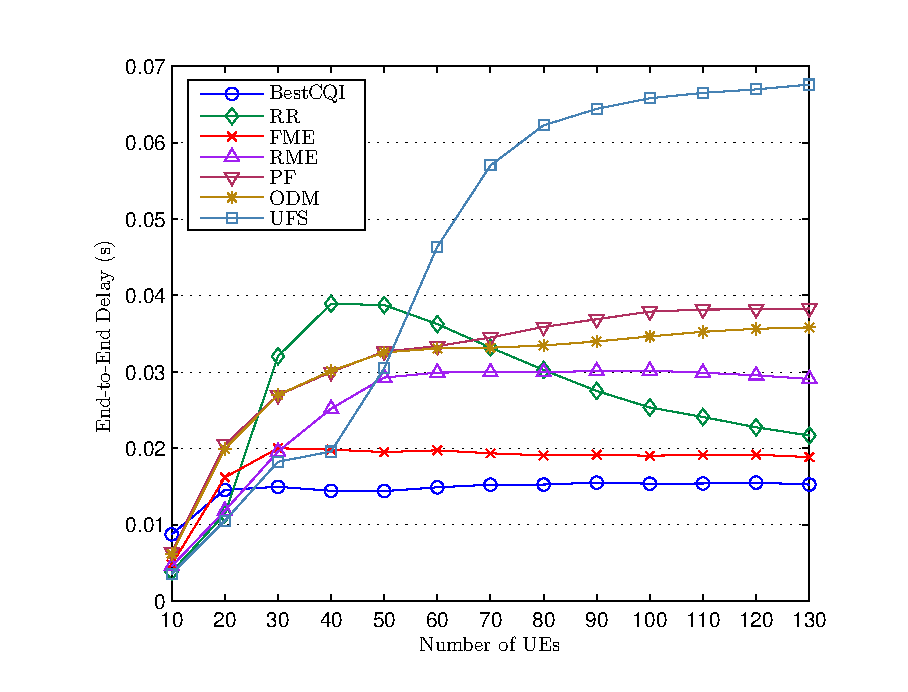
\includegraphics[%
  	scale=0.7,keepaspectratio]{figure/fixed/Delay}
}
\subfigure[\label{fig:ran_delay}隨機服務流數量下整體端點對端點延遲。]{
	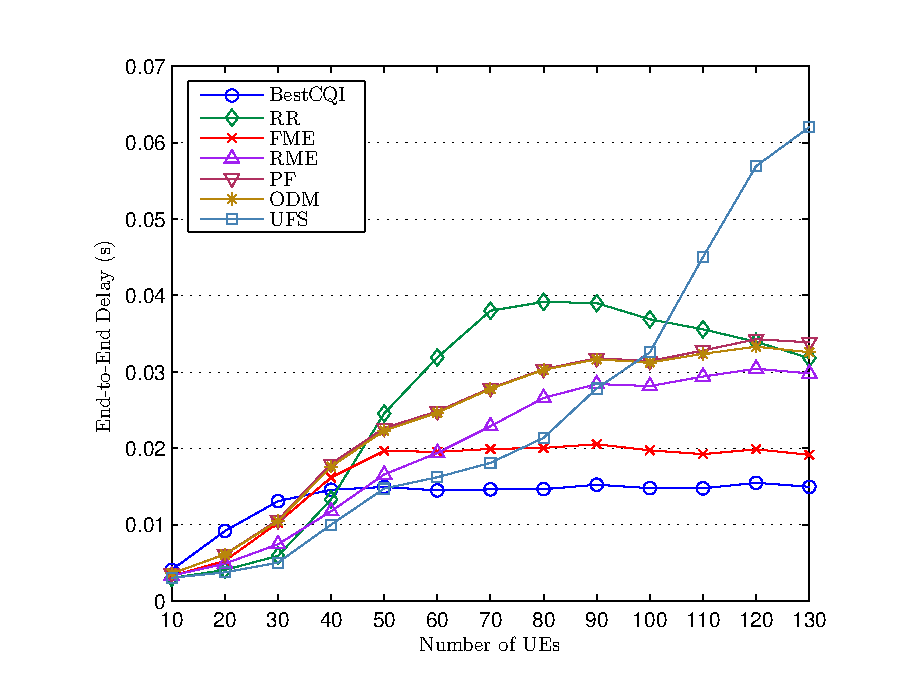
\includegraphics[%
	scale=0.7,keepaspectratio]{figure/random/Delay}
}
\caption{\label{fig:delay}不同環境中的端點對端點延遲。}
\end{figure}
\end{comment}
\clearpage
\section{各機制之封包遺失率}
封包遺失率可以分為佇列中的封包遺失率以及端點對端點的封包遺失率,本碩士論文使用的封包遺失率為端點對端點的封包遺失率,其中包含在佇列中因超過封包延遲上限而被丟棄的封包遺失率,以及在傳輸中過程中因超過封包延遲上限的封包遺失率,但是,在傳輸過程中的封包封包遺失率數值過小,可以忽略不計,故此處的封包遺失率近似等同於在佇列中的封包遺失率。當封包遺失率越低,表示越少封包在使用者裝置佇列中,因為超過封包延遲時間上限而被丟棄,排程演算法在封包遺失率上的表現越佳;反之,封包遺失率越高,表示有大量的封包在使用者裝置佇列中,因為等待時間超過封包延遲上限而被丟棄,則排程演算法在封包遺失率上的表現越差。我們提出的UFS因為考量使用者裝置內的封包延遲剩餘時間,會將資源給急迫度較高的使用者裝置,目的希望給予佇列頭端封包即將超過延遲預算上限的使用者裝置資源,降低封包在佇列中被丟棄的機率,以降低使用者裝置的封包遺失率。

由圖 \ref{fig:fix_PLR}和圖 \ref{fig:ran_PLR}可以看出,無論是在使用者裝置中存在固定服務流數量或是隨機服務流數量的環境下,我們所提出的UFS和BestCQI、RR、FME、RME、PF、ODM相比,不論當使用者裝置的數量為多少時,UFS都能達到較低的封包遺失率。由圖 \ref{fig:fix_PLR}可以發現,在固定服務流數量下,UFS的封包遺失率皆低於其他排程演算法。當使用者裝置數量為130時,UFS的封包遺失率分別比BestCQI、FME、RR、RME、PF、ODM低55\%、52\%、25\%、23\%、18\%、10\%。由圖 \ref{fig:fix_PLR}可以看出,在隨機服務流數量下,當使用者裝置數量為10時,UFS與RR、FME、RME的封包遺失率皆為0.003\%,除此之外,UFS的封包遺失率皆低於其他排程演算法。當使用者裝置數量為130時,UFS的封包遺失率分別比BestCQI、FME、RR、RME、PF、ODM低80\%、78\%、66\%、37\%、19\%、18\%。圖 \ref{fig:PLR}顯示出,我們提出的UFS在兩種不同服務流數量的環境下,封包遺失率的表現上都能優於其他排程演算法,其原因在於我們將使用者裝置的急迫性做為決策使用者裝置獲得資源優先順序的主要根據,這是和BestCQI、FME、RME、ODM等僅注重提升吞吐量的排程演算法之間的不同之處,也是我們主要希望所設計的排程演算法能發揮效果的地方。除此之外,UFS在固定服務流數量環境時的封包遺失率,會比在隨機服務流數量的環境時上升得更快,主要原因也是在於固定服務流數量時,使用者裝置之間擁有同樣種類以及數量的服務流,佇列中的封包預算剩餘時間的差異也比隨機服務流數量時的差異更小,因此UFS的急迫度影響程度降低,主要由平均配置資源度決策使用者裝置優先分配資源的順序。

在4.3節中提到,從圖 \ref{fig:delay_voip}、圖 \ref{fig:delay_video}、圖 \ref{fig:delay_web}中可以看出,BestCQI與FME排程演算法在VoIP、Video、Web服務流的端點對端點延遲都比其他排程演算法低,其主要原因為封包如果超過延遲預算時,便會在佇列中被丟棄,使封包遺失率上升,而從圖 \ref{fig:PLR}中可以發現,BestCQI與FME的封包遺失率都明顯高出其他排程演算法,可以說明有大量的封包在佇列中就被丟棄,只有少量的封包有機會因使用者裝置獲得資源而成功傳送出去,原因在於BestCQI與FME都是以通道品質為分配資源的依據,而且連續分配的方式效率不佳,一次排程中只會有少數使用者裝置配置到資源,因此,大量的封包在使用者裝置取得資源之前便超過延遲預算上限而被丟棄,使用者裝置的封包遺失率不佳。
\begin{figure}[H]
\centering
\subfigure[\label{fig:fix_PLR}固定服務流數量下的封包遺失率。]{
 	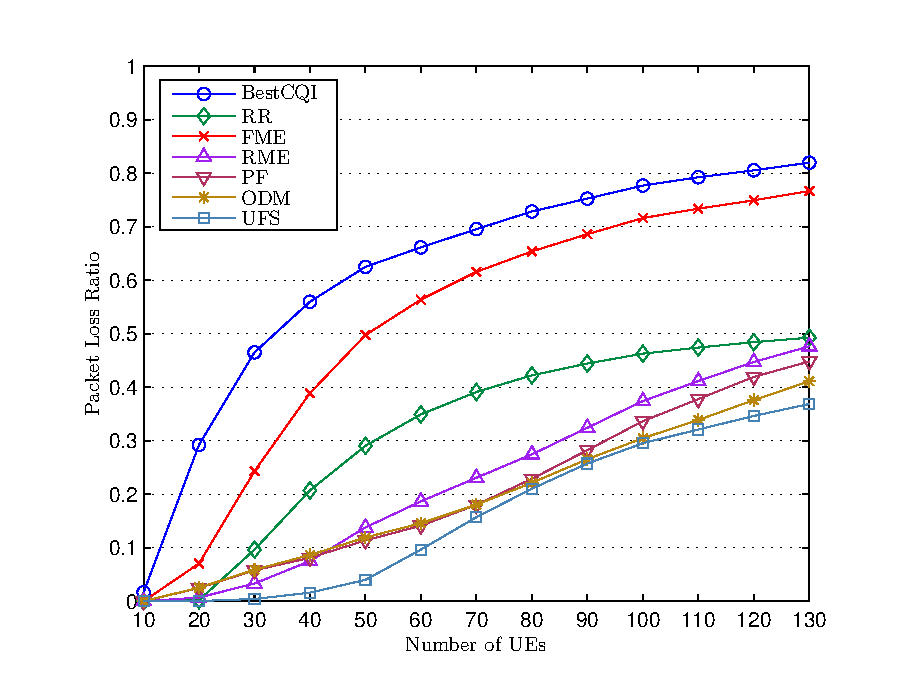
\includegraphics[%
  	scale=0.7,keepaspectratio]{figure/fixed/PLR}
}
\subfigure[\label{fig:ran_PLR}隨機服務流數量下的封包遺失率。]{
	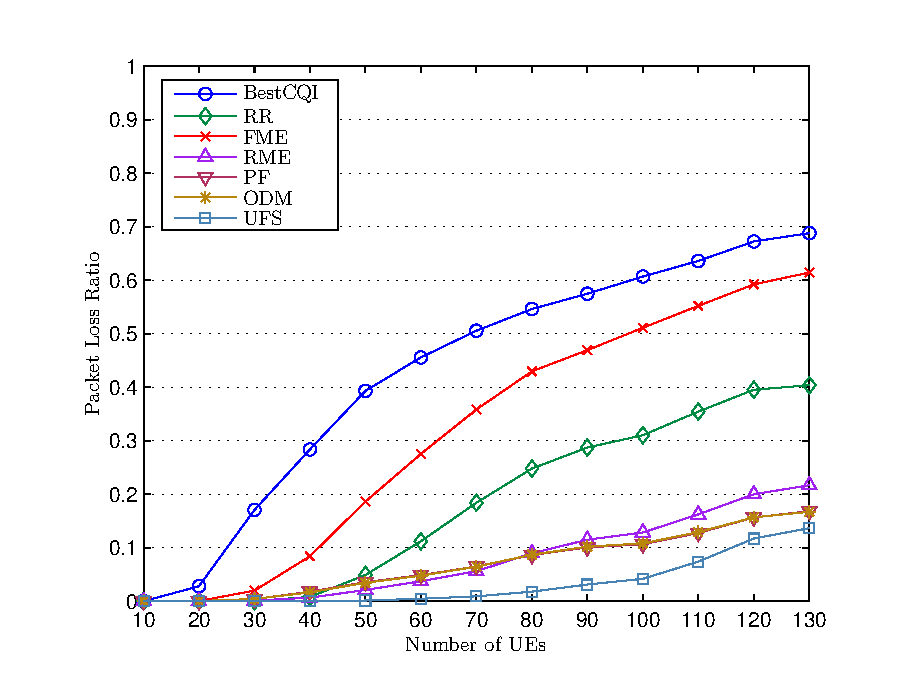
\includegraphics[%
	scale=0.7,keepaspectratio]{figure/random/PLR}
}
\caption{\label{fig:PLR}不同環境中的封包遺失率。}
\end{figure}
\begin{comment}
\begin{figure}[H]
\centering
\subfigure[\label{fig:fix_PLR}固定服務流數量下的佇列中封包遺失率。]{
 	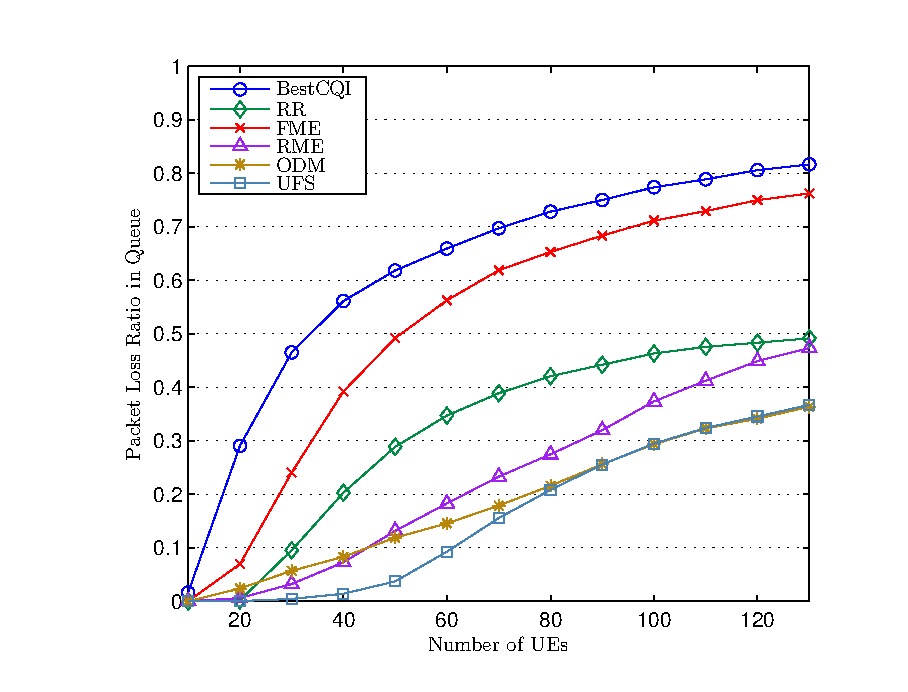
\includegraphics[%
  	scale=0.7,keepaspectratio]{figure/fixed/PLR_Queue}
}
\subfigure[\label{fig:ran_PLR}隨機服務流數量下的佇列中封包遺失率。]{
	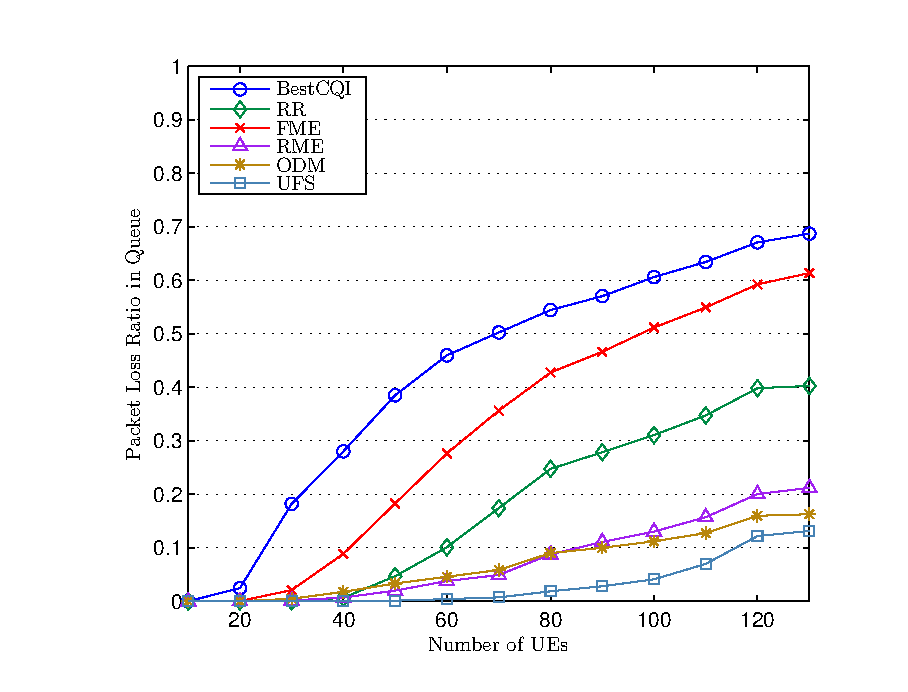
\includegraphics[%
	scale=0.7,keepaspectratio]{figure/random/PLR_Queue}
}
\caption{\label{fig:PLR}不同環境中的佇列中封包遺失率。}
\end{figure}
\end{comment}
\begin{comment} %PLR table
\begin{table}[H]
\centering
\caption{不同服務流數量下封包遺失率差異幅度表。}
\vskip 10pt
\label{tab:PLR_comp}
\begin{tabular}{|c|c|l|}
\hline
\multicolumn{1}{|l|}{} & \multicolumn{2}{c|}{UFS}              \\ \cline{2-3}
         & Fixed Flows      & \multicolumn{1}{c|}{Randomi Flows} \\ \hline
Best CQI & -99.82\% $\sim$ -55.03\% & -99.92\% $\sim$ -62.50\% 	 \\
RR       & -95.38\% $\sim$ \enskip 0.00 \%& -96.96\% $\sim$ \enskip 0.00 \% \\
FME      & -99.24\% $\sim$ -51.92\% & -99.44\% $\sim$ \enskip 0.00 \% \\
RME      & -92.22\% $\sim$ -20.57\% & -93.08\% $\sim$ \enskip 0.00 \%   \\
ODM      & -97.88\% $\sim$ -3.05\%  & -97.17\% $\sim$ -18.12\%   \\ \hline
\end{tabular}
\end{table}
\end{comment}
\clearpage
\section{各機制之公平性}
本節使用的公平性為透過公式(\ref{fairness_index})所計算而得的加權公平性,因為考量隨機服務流數量的設定不使用公式(\ref{Jain})的珍式公平性,而對於固定服務流數量的環境使用珍式公平性來評估其使用者裝置之間的公平性。公平性為從0至1的正數,公平性越接近1,表示使用者裝置之間取得資源的機會相當,排程演算法在資源的分配上對各個使用者裝置越公平;反之,公平性越接近0,表示使用者裝置中,有些使用者裝置取得資源的機會大於其他使用者裝置,造成部分使用者裝置取得較少的資源來傳輸資料,顯示排程演算法的設計在資源分配上並未照顧到足夠的使用者裝置。

從圖 \ref{fig:Fairness}可以看出,UFS在兩種服務流數量的狀況都能維持較佳的公平性。由圖 \ref{fig:Fairness}可發現,在固定服務流數量下,UFS在各使用者裝置數量上都能維持良好的公平性,並優於其他排程演算法。當使用者裝置數量為130時,UFS的公平性分別比BestCQI、FME、RME、ODM、PF、RR高出223\%、180\%、59\%、31\%、25\%、6\%,其中RR的公平性在使用者裝置數量為70後隨著使用者裝置數量而提升,主要原因在於RR分配資源時,每一個分配到的使用的裝置的資源區塊數量都是固定的;在使用者裝置數量較少時,使用者裝置分配的資源區塊數量較多,但是其中很可能包含通道品質較差的資源區塊,因此,必須使用較低的調變編碼技術,分配給使用者裝置較多的資源區塊反而會傳輸較少的資料量,造成吞吐量下降,因此,使用者裝置之間的公平性下降。由圖 \ref{fig:Fairness}可發現,在隨機服務流數量下,UFS的加權公平性可以維持在較高的數值範圍內。當使用者裝置數量為130時,UFS的加權公平性分別比FME、BestCQI、RR、RME、ODM、PF高出673\%、643\%、63\%、23\%、8\%、5\%。在公平性上UFS能優於其他排程演算法的原因在於:在排程的過程中,除了會將資源優先給較急迫的使用者裝置外,還會考量使用者裝置所獲得的平均分配過的資源區塊數量,降低過去平均獲得較多資源區塊數量的使用者裝置的優先度,讓配置過較少資源區塊的使用者裝置有更多優先分配資源的機會。而從圖 \ref{fig:ran_fairness}中也可以看出各排程演算法的線條不如圖 \ref{fig:fix_fairness}來得平滑,主要原因在於隨機分配的服務流數量環境中,每個使用者裝置所擁有的即時性服務流與非即時性服務流不盡相同,且不同使用者裝置數量之間的服務流數量亦不為等差級數般的成長,因而產生上下震盪的結果,但仍可以看出使用者裝置數量上升時,UFS相較其他排程演算法仍然維持較佳的公平性。
\begin{comment} %Fairness table
\begin{table}[H]
\centering
\caption{不同服務流數量下公平性差異幅度表。}
\vskip 10pt
\label{tab:fairness_comp}
\begin{tabular}{|c|c|l|}
\hline
\multicolumn{1}{|l|}{} & \multicolumn{2}{c|}{UFS}              \\ \cline{2-3}
         & Fixed Flows      & \multicolumn{1}{c|}{Random Flows} \\ \hline
Best CQI & 0.001\% $\sim$ +223.41\% & -0.001\% $\sim$ +642.55\% \\
RR       & -0.04\% $\sim$ +27.27\%  & \enskip -3.39\% $\sim$ +63.19\% \\
FME      & -0.08\% $\sim$ +179.51\% & \enskip -1.47\% $\sim$ +672.54\% \\
RME      & -0.07\% $\sim$ +59.11\%  & \enskip -2.29\% $\sim$ +23.22\% \\
ODM      & -0.09\% $\sim$ +30.69\%  & \enskip -5.15\% $\sim$ +24.51\% \\ \hline
\end{tabular}
\end{table}
\end{comment}
\begin{figure}[H]
\centering
\subfigure[\label{fig:fix_fairness}固定服務流數量下的公平性。]{
 	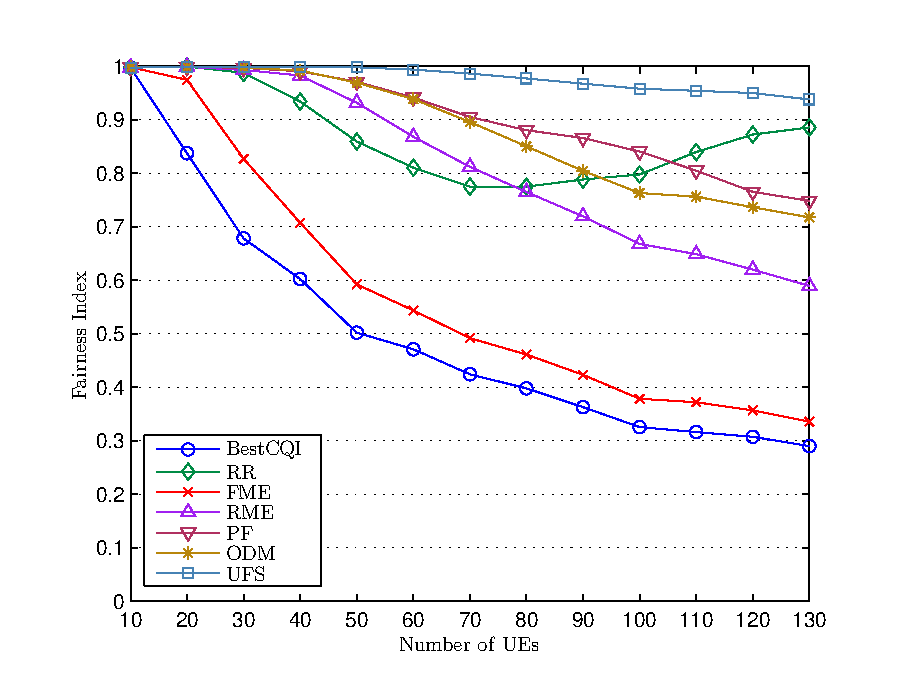
\includegraphics[%
  	scale=0.7,keepaspectratio]{figure/fixed/Fairness}
}
\subfigure[\label{fig:ran_fairness}隨機服務流數量下的公平性。]{
	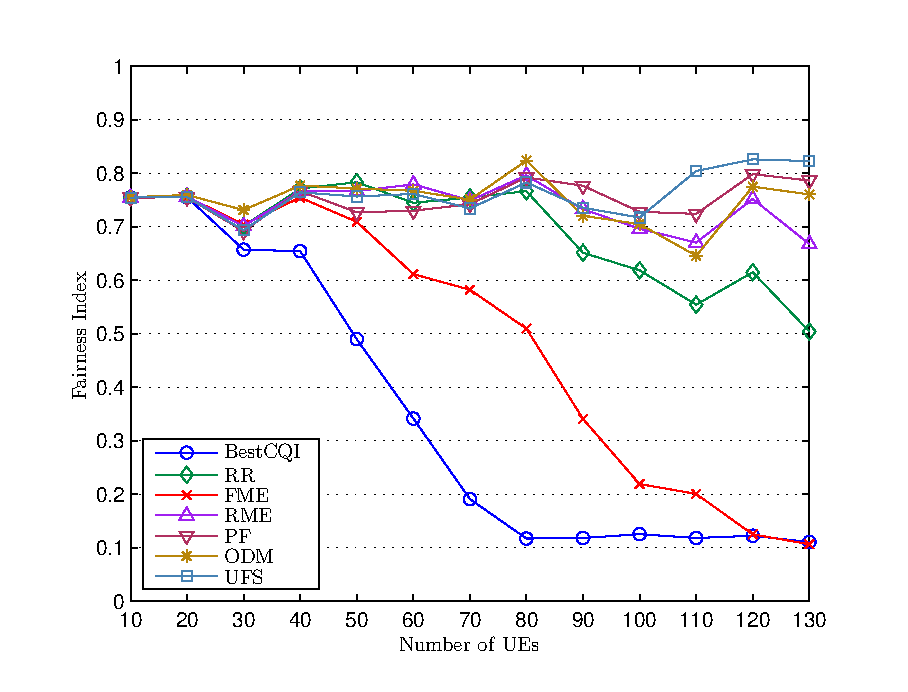
\includegraphics[%
	scale=0.7,keepaspectratio]{figure/random/Fairness}
}
\caption{\label{fig:Fairness}不同環境中的公平性。}
\end{figure}

\clearpage
\section{各機制之吞吐量}
吞吐量為系統中實際傳輸的封包量,當吞吐量越大,表示系統內全部的使用者裝置,因為資源分配得宜或是網路狀況良好,可以傳輸給基地台的資料越多,反之,若吞吐量越小,則表示可能因為資源分配或是網路狀況不佳,系統中只能傳輸少量的資料。由圖 \ref{fig:fix_Throughput}可以發現,在固定服務流數量時,UFS的吞吐量在使用者裝置數量為100以前皆高於其他排程演算法,在使用者裝置數量為110之後則僅少於RME。在使用者裝置數量為60時,UFS的吞吐量會分別比RR、BestCQI、FME、RME、ODM、PF高出234\%、159\%、118\%、34\%、20\%、19\%;在使用者裝置數量為130時,UFS的吞吐量會分別比RR、BestCQI、FME、PF、ODM高出436\%、100\%、65\%、18\%、1\%,同時比RME少15\%。其主要原因在於固定服務流數量的環境下,使用者裝置內的服務流種類以及數量固定,使得使用者裝置之間的平均封包延遲預算剩餘時間的差異小,UFS中的使用者裝置急迫性的影響下降;除此之外,在選擇優先分配資源的使用者裝置時,並不是選擇從擁有較佳的通道品質的使用者裝置開始分配資源,而是以使用者裝置的急迫度為優先,有機會會從通道品質較差的使用者裝置開始分配資源,造成較差的吞吐量。另外,RME為以提升吞吐量為目標的排程演算法,除了從擁有最佳通道品質的使用者裝置以及資源區塊開始分配外,在連續分配上同樣也以通道品質為依據,加上遞迴方式的左右分配,與BestCQI、FME、ODM等更能有效的利用資源區塊,因此在使用者裝置數量增加但能取得資源的使用者裝置數量越少時,在吞吐量上仍能優於其他排程演算法。

由圖 \ref{fig:ran_Throughput}可以看出,UFS在隨機服務流數量的環境下,在各使用者裝置數量時,吞吐量相較其他的排程演算法都有較佳的表現。當使用者裝置為130時,UFS的吞吐量分別比RR、BestCQI、FME、RME、PF、ODM高出377\%、147\%、112\%、24\%、15\%、14\%,UFS的吞吐量上優於其他排程演算法的主要原因之一在於考量封包在佇列中的平均服務流延遲預算剩餘時間;即時性的服務流(如Video服務流)的延遲預算上限比非即時性服務流(如Web服務流)低許多,使得擁有較多即時性服務流的使用者裝置比擁有較少即時性服務流的使用者裝置有更高的機率先取得資源,因而能有較高的吞吐量;此外,另外一個原因是考量了調變編碼技術的限制,會控制使用者裝置取得資源區塊的數量,使其能使用等級較高的調變編碼技術,故而能一次傳送更多的資料。
\begin{figure}[H]
\centering
\subfigure[\label{fig:fix_Throughput}固定服務流數量下的吞吐量。]{
 	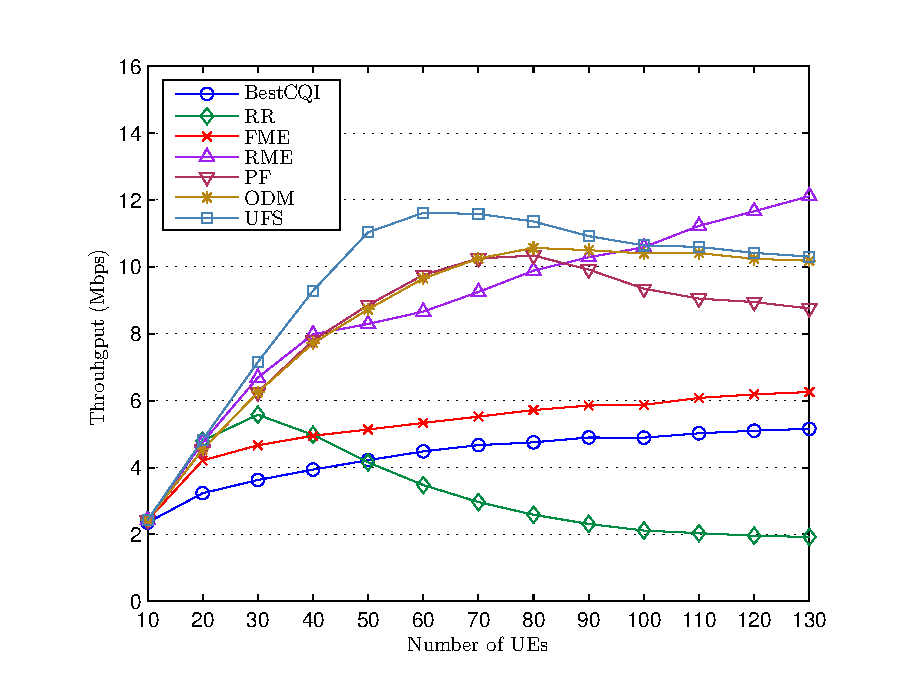
\includegraphics[%
  	scale=0.7,keepaspectratio]{figure/fixed/Throughput}
}
\subfigure[\label{fig:ran_Throughput}隨機服務流數量下的吞吐量。]{
	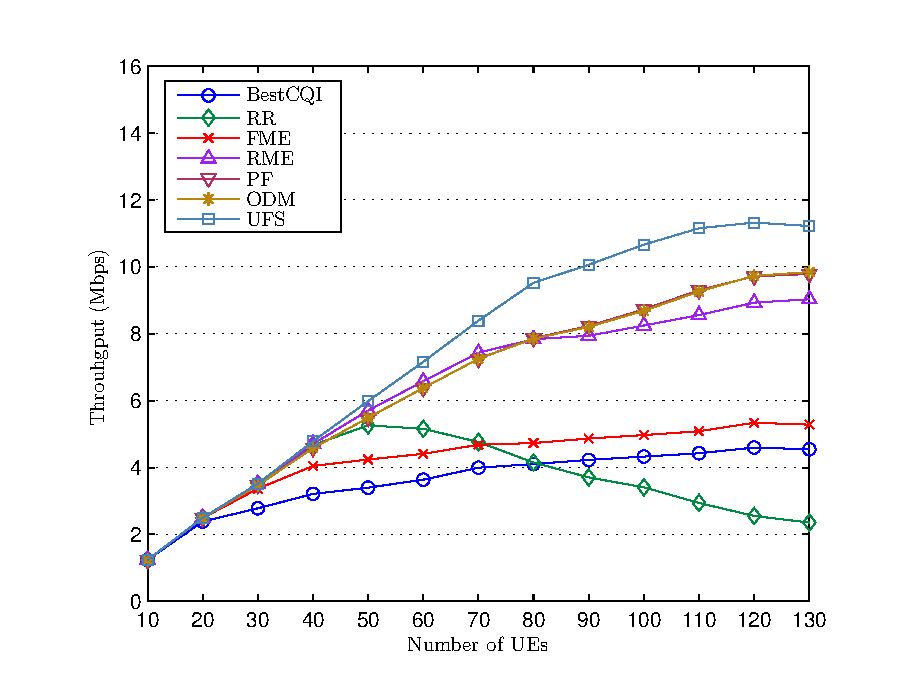
\includegraphics[%
	scale=0.7,keepaspectratio]{figure/random/Throughput}
}
\caption{\label{fig:Throughput}不同環境中的吞吐量。}
\end{figure}
\begin{comment}
\begin{table}[H]
\centering
\caption{不同服務流數量下吞吐量差異幅度表。}
\vskip 10pt
\label{tab:throughput_comp}
\begin{tabular}{|c|c|l|}
\hline
\multicolumn{1}{|l|}{} & \multicolumn{2}{c|}{UFS}              \\ \cline{2-3}
         & Fixed Flows      & \multicolumn{1}{c|}{Random Flows} \\ \hline
Best CQI & \enskip +3.04\% $\sim$ +161.77\%  & \enskip\enskip +0.01\% $\sim$ +152.07\%  \\
RR       & \enskip +0.0002\% $\sim$ +436.09\%  & -0.0008\% $\sim$ +377.04\%  \\
FME      & \enskip +0.13\% $\sim$ +117.38\%  & \quad\enskip 0.00\% $\sim$ +119.30\% \\
RME      & -14.92\% $\sim$ +34.09\%  & +0.0008\% $\sim$ +30.37\%  \\
ODM       & +0.15\% $\sim$ +26.45\%   & \quad +0.02\% $\sim$ +22.72\%  \\ \hline
\end{tabular}
\end{table}
\end{comment}

